The Precision Timed ARM (PTARM) architecture is a realization of the PRET principles on the ARM instruction set architecture\todo{Citation}. 
In this chapter we describe in detail the implementation of the timing-predictable ARM processor and the timing analysis on the architecture.
We show that with the architectural design principles of PRET, the PTARM architecture is easy analyzable with repeatable timing.
  
The architecture of PTARM follows the design principles discussed in chapter~\ref{chapter:pret}.
This includes a thread-interleaved pipeline and an exposed memory hierarchy with scratchpads and a timing predictable DRAM controller.
The ARM ISA was chosen not only due to its popularity in the embedded community, but also because it is a \emph{Reduced Instruction Set Computer} (RISC), which contains simpler instructions that allow more precise timing analysis. 
\emph{Complex Instruction Set Computers} (CSIC), such as Intel's x86\todo{citation} ISA, adds complexity to the instructions, hardware, and timing analysis.
RISC architectures typically feature a large uniform register file, use a load/store architecture, and use fixed-length instructions.
In addition, the ARM ISA contains several unique features. 
Here we list of a few.  
First, the ARM ISA does not contain explicit shifting instructions.
Instead, data-processing instructions can shift its operands before the data operation. 
This requires a separate hardware shifter in addition to the arithmetic logic unit (ALU) in the hardware.  
Second, ARM's load/store instructions contain auto-increment capabilities that can increment or decrement the value stored in the base address register.
This is done when load/store instructions use the pre or post-index addressing mode.   
This is useful to compact code that operate on data structures such as arrays or stacks. 
In addition, almost all of the ARM instructions are conditionally executed.
The conditional execution improves architecture throughput with potential added benefits of code compaction\todo{Citation}.     

ARM programmer's model specifies 16 general purpose registers (R0 to R15), with register 15 being the program counter (PC). 
Writing to R15 triggers a branch to the written value, and reading from R15 reads the current PC plus 8.
ARM has a rich history of versions for their ISA.
PTARM implements the ARMv4 ISA, without support for the thumb mode.
In addition to the predictable architecture, PTARM extends the ARM ISA with timing instructions introduced in chapter~\ref{sec:programming_models}.
We describe the implementation of these timing instructions in detail in section~\ref{sec:timing_inst_implementation} below.    

\section{Thread-Interleaved Pipeline}
\todo{discuss the term thread cycle.}
PTARM implements a thread-interleaved pipeline for the ARM instruction set.
Curretly, PTARM targets Xilinx Virtex-5 Family FPGAs, thus several design decisions were made to optimize PTARM for that FPGA family.
PTARM implements a 32 bit datapath five stage thread-interleaved pipeline.
Thread-interleaved pipelines remove pipeline hazards with by interleaving multiple threads, improving throughput and predictability. 
Conventional thread-interleaved pipelines have at least as many threads as pipeline stages to keep the pipeline design simple and maximize the clock speed.
However, Lee and Messerschmitt~\cite{lee1987pip} showed that hazards can also be removed in the pipeline even if the number of threads is one less than the number of pipeline stages.  
Increasing the number of threads in the pipeline increases each thread's latency, because threads are time-sharing the pipeline resource. 
Thus, PTARM implements a five stage thread-interleaved pipeline with four threads by carefully designing the PC writeback mechanism one pipeline stage earlier.

\begin{figure}[b]
  \vspace{-20pt}
  \begin{center}
    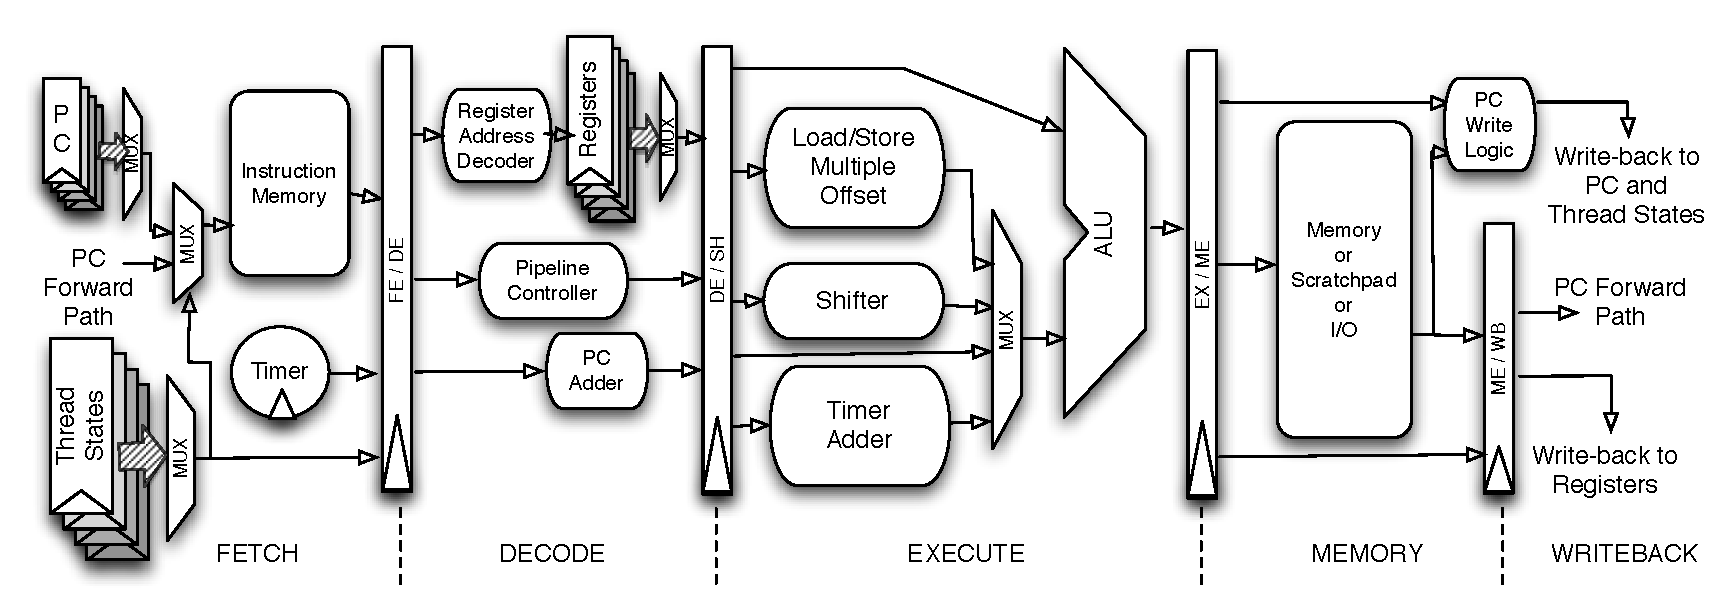
\includegraphics[scale=.54]{figs/ptarm_pipeline_five_stage}
  \end{center}
  \vspace{-20pt}
  \caption{Block Level View of the PTARM 5 stage pipeline}
  \label{fig:ptarm_pipeline_five_stage}
\end{figure}

Figure~\ref{fig:ptarm_pipeline_five_stage} shows a block diagram view of the pipeline. 
Some multiplexers within the pipeline have been omitted for a clearer view of the hardware components that make up the pipeline.
There contains four copies of the Program Counter(PC), Thread States, and Register File.
The register file has 3 read ports and 1 write port.
Most of the pipeline design follow the five stage pipeline described in Hennessy and Patterson\todo{citation}, with the five stages in the pipeline being \emph{Fetch}, \emph{Decode}, \emph{Execute}, \emph{Memory}, and \emph{Writeback}.
We briefly describe the functionality of each stage, and leave more details to section~\ref{sec:ptarm_instructions}, where the instruction implementations are presented.

The \emph{fetch stage} of the pipeline selects the correct PC according to which thread is executing, and passes the address to instruction memory. 
A simple 2 bit ($log(n)$) up-counter is used to keep track of which thread current to fetch.
This reduces the time and space overhead of context switching close to zero. 
The PC forward path is used when an instruction loads to R15, which causes a branch to the value loaded from main memory.  
We will discuss the need for the forwarding path below when the \emph{memory stage} is described.
The \emph{timer} implements the \emph{platform clock} used by the timing instructions.
In addition, it contains the hardware logic that registers and checks for timer expiration exceptions for each thread.
A 64 bit timestamp in nanoseconds is associated with each instruction when it begins execution in the pipeline.
This 64 bit timestamp is latched together from the \emph{timer} in the fetch stage, and is kept with the instruction for the duration of its execution. 

The \emph{decode stage} contains the \emph{pipeline controller} that decodes instructions and determines the pipeline control signals to be propagated down the pipeline.
Most of ARM instructions are conditionally executed, so the pipeline controller also checks the condition bits against the processor state condition codes to determine whether the instruction is to be executed or not.  
Typically, \emph{pipeline controllers} needs to keep track of all instructions currently executing in the pipeline, to detect the possibility of pipeline hazards and handle them correspondingly.
However, from the \emph{decode} stage of our thread-interleaved pipeline, other instructions executing in the pipeline are instructions from other threads.
Thus, the controller logic is greatly simplified because no hazard checking from in-flight instructions is required.  
A small decoding logic, the \emph{register address decoder}, is inserted in parallel with the controller to decode the register addresses from the instruction bits.  
In typical RISC instruction sets, such as MIPS, the register operands have a fixed location for all instruction encodings.
Thus, they can directly be passed into the register file before decoding.   
However, in the ARM instruction set, certain instructions encode the register read address at different bit locations of the instruction.
For example, data-processing register shift instructions and store instructions reads a third operand from the register that are at encoded at different bit locations.
Thus, a small register address decoding logic is inserted for a quick decoding of the register addresses from the instruction bits.
\todo{Check if the register can be read from two different stages, thus removing the need for a register decoder logic. If rm and rn always remain the same, then we can read rs (rd for store) a stage later. }

The \emph{PC Adder} is the logic block that increments the PC. 
Single threaded pipelines need to increment the PC immediately in the fetch stage to prepare for instruction fetch the next processor cycle.  
For thread-interleaved pipelines, the next PC from the current thread is not needed until several cycles later, so there is no such restriction.
In addition to outputting the current PC incremented by 4, the \emph{PC Adder} also outputs the value of the current PC incremented by 8.
In the ARM ISA, instructions that use R15 as an operand actually read the instruction PC plus 8, instead of the instruction PC, as the value of the operand.
This is designed for the convenience of architecture implementation. 
Typically in pipelines, instructions take 2 cycles (fetch and decode) before it enters the execute stage. 
For single-threaded pipelines, the program counter has likely been incremented by 8 at the time the instruction enters the execute stage.
By using $instruction\_pc+8$ as the operand value, the hardware implementation can directly use the processor PC currently in the fetch stage, without compensating for the two increments that occurred. 
However, for thread-interleaved pipelines, we need to explicitly calculate $instruction\_pc+8$, because the PC for each thread is not incremented every processor cycle, but incremented once every round-robin scheduling cycle.
Since $instruction\_pc+8$ could be used as a data operand needed in the execute stage, the \emph{PC Adder} in placed in the \emph{decode} stage.  

The \emph{execute stage} contains execution units and multiplexers that select the correct operand and feeds it to the ALU.  
The ARM ISA assumes an additional shifter to shift the operands before data operations, so a 32 bit \emph{Shifter} is included.
The 32 bit \emph{ALU} does most of the logical and arithmetic operations, including data-processing operations and branch address calculations.
The \emph{Load/Store Multiple Offset} logic block calculates the offset for load/store multiple instructions.
Load/store multiple instructions use a 16 bit vector to represent each of the 16 general purpose registers.
Memory operations are done only on the registers whose corresponding bit value is set in the bit vector.
The memory addresses of each memory operation is derived from the base register and an offset. 
%The an offset is added to the base memory address for the instruction, and that offset depends on how many bits are set.
The \emph{Load/Store Multiple Offset} logic block calculates this offset according to the bit count of the remaining bit vector during load/store multiple instructions.
The \emph{Timer Adder} is a 32 bit add/subtract unit used with the \emph{ALU} to compare 64 bit timestamps for timing instructions. 
Specifically, \delayuntil\ requires the comparison of two 64 bit timestamps every thread cycle, thus the additional \emph{Timer Adder} is added to accomplish that.  
The implementation details of \delayuntil\ is described in section~\ref{sec:timing_inst_implementation}.

\begin{wrapfigure}{r}{0.5\textwidth}
  \vspace{-20pt}
  \begin{center}
    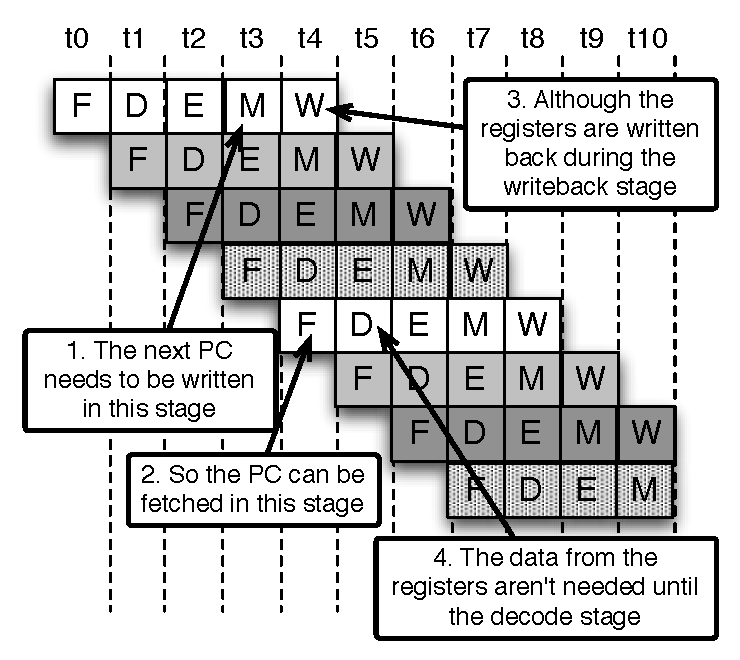
\includegraphics[scale=.65]{figs/four_thread_pipeline}
  \end{center}
  \vspace{-3mm}
  \caption{Four thread execution in PTARM}
  \label{fig:four_thread_pipeline}
  \vspace{-10pt}
\end{wrapfigure}      
     
The \emph{memory stage} issues the memory operations and writes back the PC and thread states.
The PC and thread states are written back a stage early to allow us to interleave four threads in our five stage pipeline, instead of five.
This improves the latency of individual threads. 
When four threads are interleaved through a five stage pipeline, if the PC is written back in the \emph{writeback stage}, then the next instruction fetch for the thread would not see the updated PC in time for its instruction fetch. 
Figure~\ref{fig:four_thread_pipeline} illustrates this by showing an execution sequence of the four thread five stage thread-interleaved pipeline in PTARM.
Each cycle, the instructions in the \emph{fetch} and \emph{writeback} stages belong to the same thread.
Thus, committing the PC in the \emph{writeback stage} would cause a control hazard because the updated PC would not observed by the concurrent instruction fetch.
For most instructions, including branch instructions, the next PC is known before the memory stage, so moving the PC commit one stage earlier does not cause any problems.  
The \emph{PC Write Logic} updates the next PC, depending on the instruction, and whether an exception occurred or not.
Section~\ref{subsec:exception_handling_in_ptarm} describes the hardware mechanism for handling exceptions in PTARM. 
Normally, PC+4 from the \emph{PC Adder} or the results from the \emph{ALU} is used to update the PC.

Whenever instructions write to R15 (PC), the control flow of the program branches to the value written to R15.
Data processing instructions that write to R15 have its results computed by the \emph{execute stage}, ready to be committed as the new PC in the \emph{memory stage}.    
However, a load instruction that loads to R15 will not know the branch target until after the memory read.
Thus, a PC forwarding path is added to forward the results back from memory as the fetched PC if a load instruction loads to R15.  
The forwarding path does not cause any timing analysis difficulties because the statically the forwarding path is only and always used when a load instruction loads to R15, which can be statically determined. 
Also, this causes no stall in the pipeline, and does not effect the timing of any following instructions.
We describe the implementation more details in section~\ref{sec:load_to_pc}. 

The \emph{writeback stage} simply writes back the results from memory or the \emph{ALU} to the correct registers.
Writing back to registers in the \emph{writeback stage} does not cause data hazards even if there are only four threads, because the data from registers are not read until the following \emph{decode stage}.
Figure~\ref{fig:four_thread_pipeline} shows that the two stages do not overlap in the same cycle, thus causing no hazards.  

\section{Memory Hierarchy}
\label{sec:ptarm_memory}
The memory hierarchy of PTARM is exposed in software, as discussed in section~\ref{section:memory_system}.
This allows for a more predictable and analyzable memory access latency from the architecture. 
The memory hierarchy is composed of regions reserved for the boot code, the instruction and data scratchpads, a 512MB DRAM Module, and the memory mapped I/O, all occupying separate address regions.
Figure~\ref{fig:ptarm_memory_layout} shows the memory address regions reserved for each memory type.
Both the boot code and scratchpads are synthesized to dual-ported block RAMs on the FPGA, and provide deterministic single cycle access latencies.

\begin{wrapfigure}{r}{0.35\textwidth}
  \vspace{-30pt}
  \begin{center}
    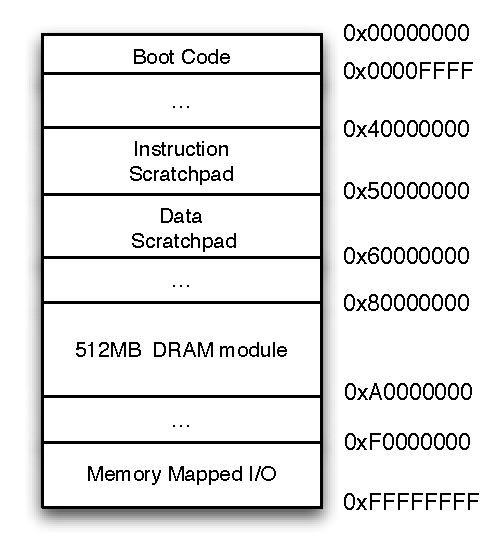
\includegraphics[scale=.65]{figs/ptarm_memory_layout}
  \end{center}
  \vspace{-5mm}
  \caption{Memory Layout of PTARM}
  \label{fig:ptarm_memory_layout}
\end{wrapfigure} 

\subsection{Boot code}
The \emph{boot code} region contains initialization and setup code for PTARM. 
This includes the exception vector table, which stores entries used jump to specific exception handlers for the different exceptions.
The specific table entries and layout is explained in section~\ref{subsec:exception_handling_in_ptarm}. 
Non-user registered exception handlers and the exception setup code are also part of the boot code .
When PTARM resets, all threads begin execution at address 0x0, which is the \emph{reset} exception entry in the exception vector table.
The \emph{reset} exception handler will setup each thread's execution state, including the stack, which is allocated on the data scratchpad.
Then the handler transfers control flow to the user compiled code for each thread.  
Dedicated locations in the boot code is reserved for user-registered exception handlers, these entries can be modified programmatically. 
For example, a location is reserved to store the location of a user registered timer expire exception handler.

\subsection{Scratchpads}
The scratchpads replace caches as the fast-access memory in our memory hierarchy.   
The partition of instruction and data scratchpads between threads can be configured into different schemes depending on the application.   
For embedded security applications, such as encryption algorithms, partitioning the scratchpads into private regions in hardware for each thread might be desired to prevent cross-thread attacks.
In section~\ref{sec:app_side_channel_attack} we discuss the security implications and how partitioning the scratchpad can defend against timing side-channel attacks that exploit underlying shared resources.
On the other hand, on applications with collaborative hardware threads, sharing the scratchpad could provide flexibility for the memory allocation scheme~\cite{Suhendra:2010:SAC:1734206.1734210} of scratchpads and communication between hardware threads.
This opens opportunities to optimize system performance, instead of just individual threads.  
Hybrid schemes can also be used that privatizes a hardware thread for security, and allows other threads for collaboration.  

\subsection{DRAM}
\label{sec:ptarm_dram_integration}
PTARM interfaces with a $512MB$ DDR2 $667MHZ$ DRAM memory module (Hynix HYMP564S64CP6-Y5). 
All access to the DRAM goes through the predictable DRAM controller described in section~\ref{sec:pret_dram_controller}.
The DRAM controller privatizes the DRAM banks into four resources, which we assign to each thread in our pipeline. 
This removes bank access conflicts and gives us predictable memory access latencies to the DRAM.
The pipeline interacts with the frontend of the DRAM controller, which routes requests to the correct request buffer in the backend, and manages the insertion of row-access refreshes to ensure the refresh constraint is met.   
In conventional memory architectures where the hierarchy is hidden, the processor interacts with DRAM indirectly by the filling and writing back of cache lines.
In our memory system, the processor can directly access the DRAM through load and store instructions to the distinct memory regions of the DRAM.
In addition, each hardware thread is also equipped with a direct memory access (DMA) unit, which can perform bulk transfers between the scratchpads and the DRAM.
Figure~\ref{fig:pretintegration} shows the integration of PTARM with the DMA units, memory controller and DRAM.  

\begin{figure}
\noindent\makebox[\textwidth]{
\begin{minipage}[b]{0.55\linewidth}
 \begin{center}
  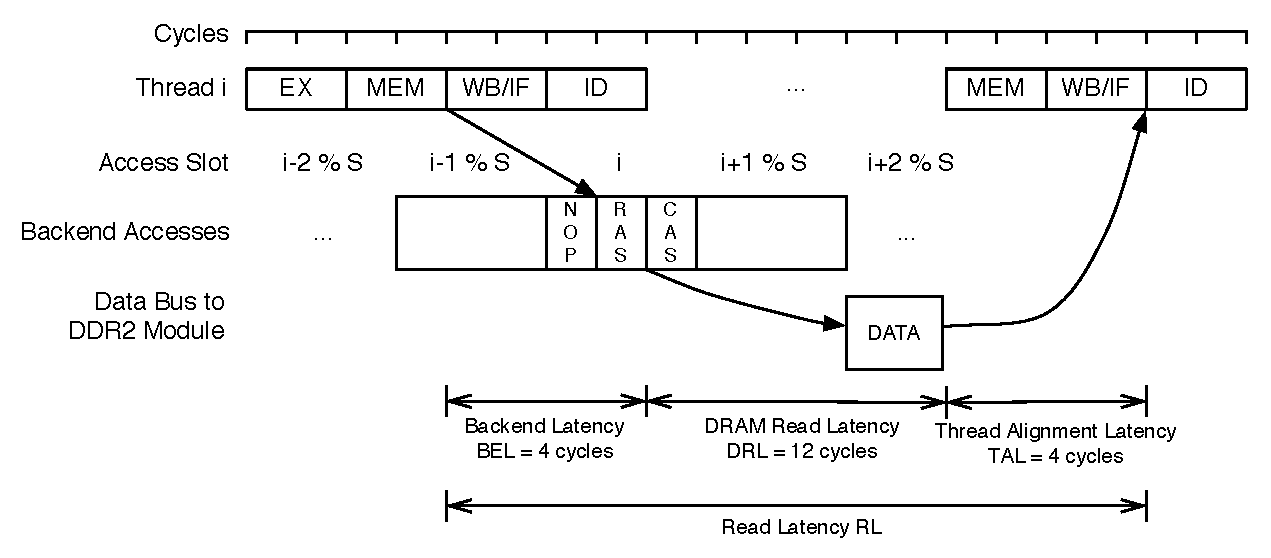
\includegraphics[scale=.4]{figs/readlatency}
  \end{center}
  \vspace{-3mm}
  \caption{Example load by thread $i$ in the thread-interleaved pipeline.}
  \label{fig:readlatencyderivation}
\end{minipage}
\hspace{3mm}
\begin{minipage}[b]{0.45\linewidth}
  \begin{center}
  	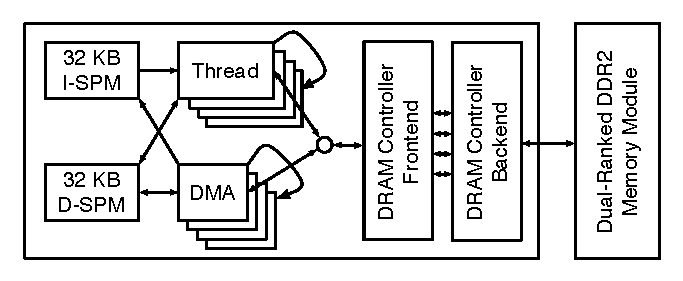
\includegraphics[scale=.6]{figs/pret-integration}
  \end{center}
    \vspace{-3mm}
  \caption{Integration of PTARM core with DMA units, PRET memory controller and dual-ranked DIMM~\cite{ReinekeLiuPatelKimLee11_PRETDRAMControllerBankPrivatizationForPredictability}.}
\label{fig:pretintegration}
\end{minipage}
}
\end{figure}

When DRAM is accessed through load (read) and store (write) instructions, the memory requests are issued directly from the memory stage of pipeline.
The request is received from the frontend of the memory controller, and placed in the correct request buffer. 
Depending on the alignment of the pipeline and the backend, it takes a varying number of cycles until the backend generates corresponding commands to be sent to the DRAM module.
After the read has been performed by the DRAM and has been put into the response buffer, again, depending on the alignment of the pipeline and the backend, it takes a varying number of cycles for the corresponding hardware thread to pick up the response.
Figure~\ref{fig:readlatencyderivation}, illustrates the stages of the execution of an example read instruction in the pipeline.
In~\cite{ReinekeLiuPatelKimLee11_PRETDRAMControllerBankPrivatizationForPredictability} we derive the access latencies from the alignment and show that it is either 3 or 4 thread cycles.    
We leverage this misalignment of the pipeline and backend to hide the refresh latency from the front end. 
When a refresh is scheduled for the DRAM resource, if no memory request is in the request buffer, the refresh is serviced.
As mentioned in section~\ref{sec:pret_dram_controller}, if a refresh conflicts with a pipeline load or store, we push back the refresh till after the load or store. 
In this case, the pushed back refreshes become invisible:   
as the pipeline is waiting for the data to be returned and takes some time to reach the memory stage of the next instruction, it is not able to use successive access slots of the backend, and thus it does not observe the refresh.

Whenever a DMA transfer is initiated, the DMA unit uses the thread's request buffer slot to service DMA requests to/from the scratchpad. 
Thus, while a DMA transfer is initiated, the thread gives up access to the DRAM to the DMA unit.
During this time, the thread can continue to execute and access the scratchpad regions that is not being serviced by the DMA request. 
This is possible because scratchpads are dual-ported, allowing a DMA unit to access the scratchpads simultaneously as its corresponding hardware thread.
If at any point the thread tries to access the DRAM, it will be blocked until the DMA transfer completes.
Similarly, accesses to the region of the scratchpad being serviced by the DMA will also stall the hardware thread\footnote{This does not affect the execution of any of the other hardware threads.}.
The DMA units can fully utilize the bandwidth provided by the backend because unlike accesses from the pipeline, they suffer the no alignment losses.
When refreshes conflict with a DMA transfer, we push back the first refresh and schedule one at the end of the DMA transfer. 
This can be seen as shifting all refreshes, during the DMA transfer, back by $63$ slots or to the end of the transfer.
More sophisticated schemes would be possible, however, we believe their benefit would be slim.
With this scheme, refreshes scheduled within DMA transfers are predictable so the latency effects of the refresh can be easily analyzed, which we derive in~\cite{ReinekeLiuPatelKimLee11_PRETDRAMControllerBankPrivatizationForPredictability}.

\paragraph{Store Buffer}
\label{sec:ptarm_dram_store_buffer}
Stores are fundamentally different from loads in that a hardware thread does not have to wait until the store has been performed in memory.
By adding a single-place store buffer to the frontend, we can usually hide the store latency from the pipeline.
Using the store buffer, stores to DRAM that are not preceded by other memory operations to DRAM can appear to execute in a single thread cycle.
%By \emph{thread cycle}, we denote the time it takes for an instruction to pass through the thread-interleaved pipeline.
Otherwise, the store will observe the full two thread cycle latency to store to DRAM.
A bigger store buffer would be able to hide latencies of more successive stores at the expense of slightly increasing the complexity of timing analysis.

\subsection{Memory Mapped I/O}
%talk about the I/O memory region, and how the protocol is implemented to determine if memory access is completed yet
Currently PTARM implements a primitive I/O bus for communicating with external inputs and outputs.
Access to the bus occurs in the memory stage of the pipeline, by accessing the memory mapped I/O region with memory instructions.
I/O devices snoop the address bus to determine whether the pipeline is communicating with it.
The I/O bus is shared by all threads in the thread-interleaved pipeline, thus, in addition to address and data, a thread ID is also sent out for potential thread-aware I/O devices. 
In section~\ref{sec:ptarm_vhdl_soft_core} below we describe the several I/O components that are connected to our PTARM core.
Currently all I/O devices interface with the processor through single cycle memory mapped I/O control registers to prevent bus contention between threads.
In order to ensure predictable access times to all I/O devices, a timing predictable bus architecture must be implemented.   
Several timing predictable bus architectures~\todo{cite} have been proposed and can be interfaced with PTARM. 
A predictable thread-aware I/O controller is also needed to ensure data from the I/O devices are read by the correct thread, and contention is properly managed.
These issues present future research opportunities -- to interface a timing predictable architecture with various I/O devices while maintaining its timing predictability.  

\section{Exceptions}
\label{subsec:exception_handling_in_ptarm}
When exceptions occur in a single threaded pipeline, the whole pipeline must be flushed because of the control flow shift in the program. 
The existing instructions in the pipeline immediately become invalid, and the pipeline fetches instructions from an entry in the exception vector table. 
The exception vector table stores entries that direct the control flow to the correct exception handling code.  
The table is part of the boot code, and its contents are shown in table~\ref{tab:exception_vector_table}.
The timer expired exception entry is added with our timing extensions to the ISA, and is triggered when a user registered timestamp with \exceptiononexpire\ expires.  
\begin{table}[h]
\noindent\makebox[\textwidth]{%
\begin{smalltabular}{ | l | l | p{6cm} | }
  \hline                        
  Address & Exception Type &  Description \\ \hline
  0x0 & Reset & \\ \hline 
  0x4 & Undefined instructions &  \\ \hline 
  0x8 & Software Interrupt (SWI) & \\ \hline
  0xC & Prefetch Abort & \\ \hline
  0x10 & Data Abort & \\ \hline
  0x18 & Interrupt (IRQ) & \\ \hline
  0x1C & Timer Expired & \\ \hline
\end{smalltabular}}
\vspace{1mm}
\caption{Exception vector table in PTARM}
\label{tab:exception_vector_table}
\end{table}

In the PTARM thread-interleaved pipeline, exceptions are separately managed for each hardware thread.  
All threads are designed to be temporally isolated in the PTARM thread-interleaved pipeline.  
Thus, an exception that triggers on one thread must not effect the execution of other threads in the pipeline.
In PTARM, any exceptions that occur during execution propagate down the pipeline with the instruction.
The exception is checked and handled before modifying any states, such as the PC, CPSR, register, memory, of the thread.  
When an exception is detected, the current instruction execution is ignored, and the PC and thread states are updated to handle the exception.   
%The program state register bits are updated to reflect an exception occurrence.  
According to the exception type, the PC is redirected to the corresponding entry in the exception vector table. 
The current PC is to store in the link register (R14), so the program can re-execute the halted instruction if desired.
%The \emph{writeback stage} to detects exceptions   
%If the exception is generated from after a memory access and detected in the writeback stage, the PC forwarding path is used to fetch the exception vector entry for data memory exceptions. 
%Note that it is up the each exception handler to save the register states and stack of the program.  

\begin{wrapfigure}{r}{0.5\textwidth}
  \vspace{-30pt}
  \begin{center}
    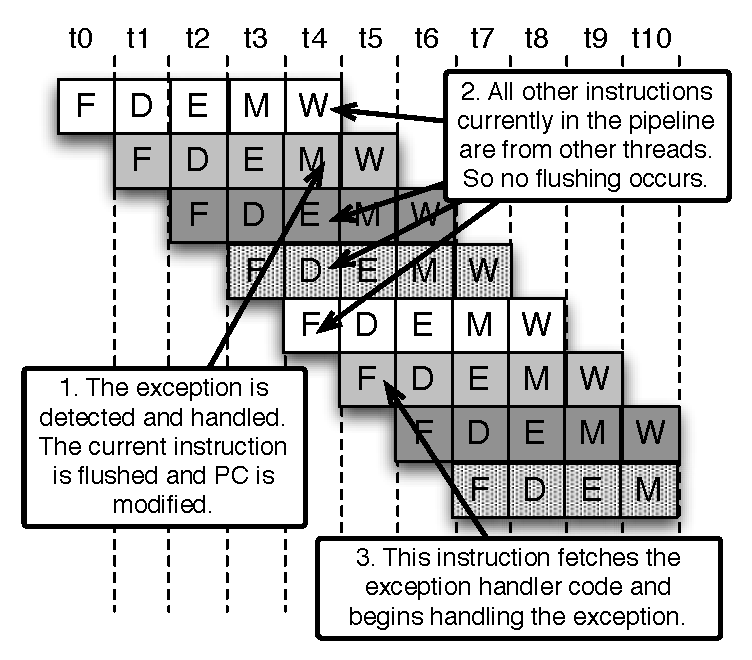
\includegraphics[scale=.65]{figs/exception_handling_pipeline}
  \end{center}
  \vspace{-3mm}
  \caption{Handling Exceptions in PTARM}
  \label{fig:exception_handling_pipeline}
  \vspace{-10pt}
\end{wrapfigure}

None of the other instructions executing in the pipeline are flushed when an exception occurs. 
As shown in figure~\ref{fig:exception_handling_pipeline}, the instructions executing in other pipeline stages belong to other threads, so no flushing of the pipeline is required because no instruction was speculatively executed.
This limits the timing affects of exceptions to only one thread, as the timing behavior of other threads in the pipeline are unaffected.
From the hardware, only a one thread cycle overhead is induced. 
In this thread cycle, the current instruction does not complete its execution, but instead the pipeline updates the thread states to reflect the exception.   
In the next thread cycle, the thread will already be executing instructions to handle the exception.

For longer latency instructions that modify the program state, exceptions can cause an inconsistent view of the program state when an exception occurs during execution.   
For example, a \timerexpired\ exception could occur in the middle of a memory instruction to the DRAM region.
In this case, we cannot cancel the memory request abruptly because the memory request is handled by the external DRAM controller, and possibly already being serviced by the DRAM.
If the memory instruction is a load, the results can be simply disregard.
But if the instruction is a store instruction, we cannot cancel the store request that is writing data to the memory.
The programmer must disable interrupts before writing to critical memory locations that require a consistent program state.

Besides an inconsistent program state, interrupting a memory instruction can also complicate the interaction between the pipeline and DRAM controller.
The DRAM controller, with a request buffer of size one, does not queue up memory requests.
This normally is not an issue because our pipeline does not reorder instructions or speculatively execute when there are outstanding memory requests.
However, if a memory instruction is interrupted, the pipeline flushes the current instruction, and control flow directly jumps the exception vector table, which directs the program to execute the corresponding exception handler. 
If instructions immediately following the exception access the DRAM, a new memory request would be issued to the DRAM controller that is still servicing the previous request prior to the exception.
The new memory request would then need to be queued until the previous ``canceled'' memory request completes before it can begin being serviced.
This creates timing variability for exception handlers, because the latency of initial load instructions would vary depending on the instruction interrupted by the exception. 
Because it is very difficult to statically analyze the exact instruction an exception would interrupt, it will be difficult to predict when this timing variance would occur.    

To achieve predictable and repeatable timing for exception handlers, we leverage the exposed memory hierarchy to ensure sufficient time has lapsed for the DRAM controller to finish servicing any potential memory requests, before any instructions in the exception handlers access the DRAM.
In PTARM, the worst-case memory latency for the DRAM backend is 4 thread cycles, so we need to ensure that the instructions executed during the first 3 thread cycles after an exception does not access the DRAM.
The exception vector table and the exception handler setup code are all part of the boot code synthesized to dual-ported BRAMs, thus instruction fetching is guaranteed to avoid the DRAM.
The exception vector entries contain only contain branch instructions, which also does not access the DRAM.
We statically compile the data stack onto the data scratchpad, so any stack manipulations that occurs also avoids the DRAM.
Thus, the exception handling mechanism in PTARM is timing predictable and repeatable. 
In section~\ref{sec:exception_timing_example} we will show an example to demonstrate this.  

Currently PTARM does not implement an external interrupt controller to handle external interrupts. 
But when implementing such an interrupt controller, each thread should be able to register specific external interrupts that it handles.
For example, a hard real-time task could be executing on one thread, while another task without timing constraints is executing on another thread waiting for an interrupt to signal the completion of a UART transfer.
In this case, the thread running the hard real-time task should not be interrupted when the UART interrupt occurs.
Only the specific thread handling the UART transfers should be interrupted by this interrupt.  
Thus, we envision a thread-aware interrupt controller that allows each thread to register specific interrupts to handle.

\section{Instruction Details}
\label{sec:ptarm_instructions}
In this section we present details on how each instruction type is implemented to show how each hardware block in the pipeline shown in figure~\ref{fig:ptarm_pipeline_five_stage} is used.
We will go through different instruction types and discuss the timing implications of each instruction in our implementation.
   
\subsection{Data-Processing}
We begin by explaining how data-processing instructions are implemented.
These instructions are used to manipulate register values by executing register to register operations. 
Most data-processing instructions take two operands.
The first operand is always a register value.
The second operand is the shifter operand, which could be an immediate or a register value.
Both can be shifted to form the final operand that is fed into the ALU.
Figure~\ref{fig:data_processing_pipeline_implementation} explains how data-processing instructions are executed through the pipeline.

\begin{figure}[h]
  \vspace{-15pt}
  \begin{center}
    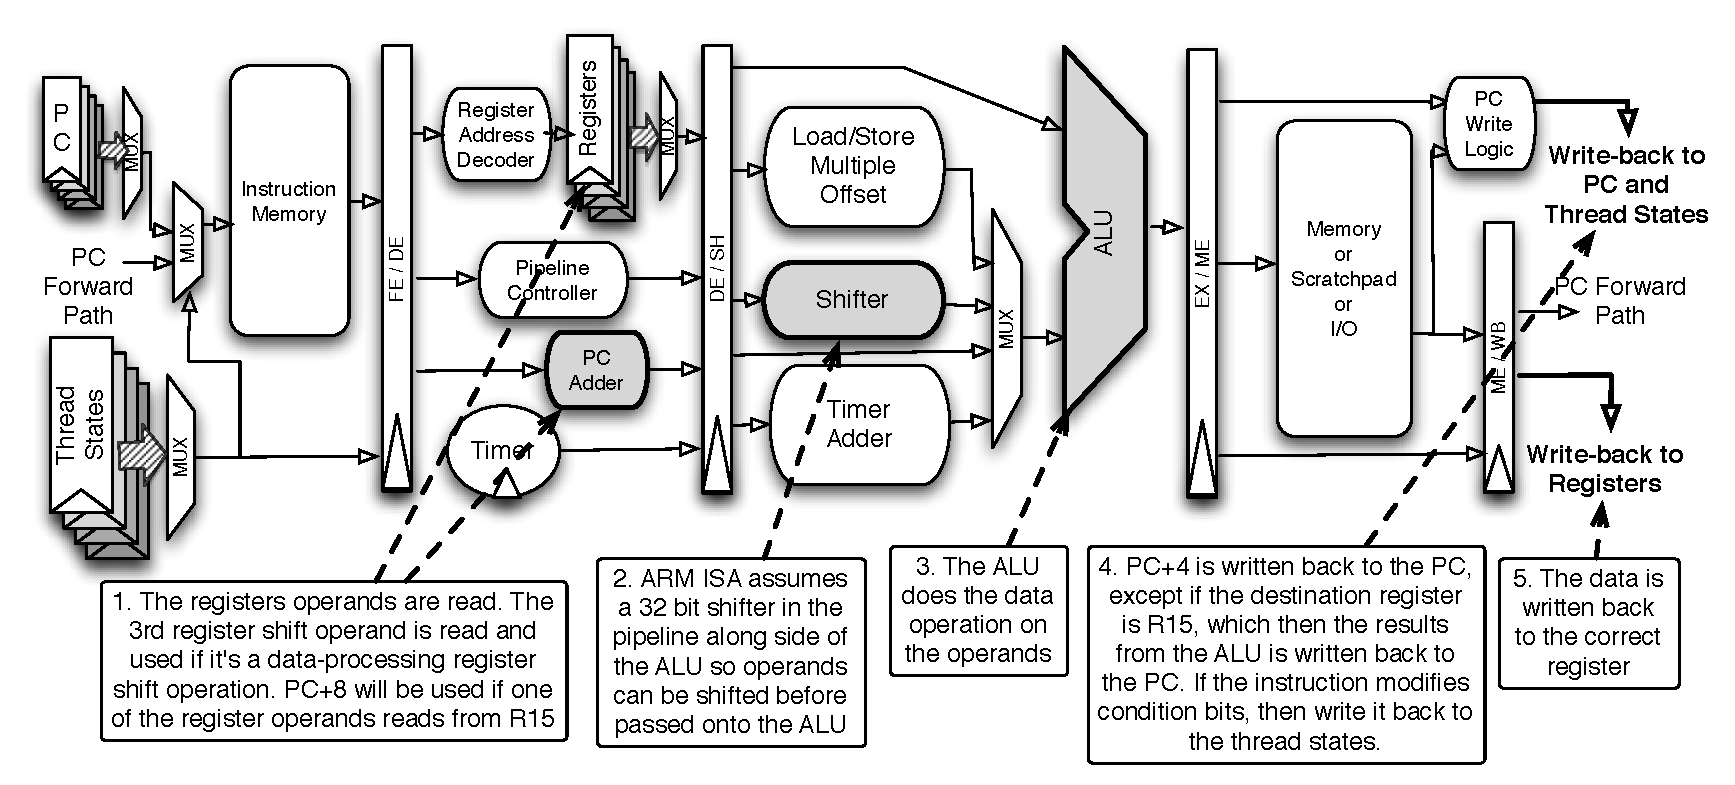
\includegraphics[scale=.54]{figs/data_processing_pipeline_implementation}
  \end{center}
  \vspace{-3mm}
  \caption{Data Processing Instruction Execution in the PTARM Pipeline}
  \label{fig:data_processing_pipeline_implementation}
\end{figure}

The execution of data-processing instructions is fairly straightforward.
Operands are read from the register file or instructions bits.
They are shifted if required, then sent to the ALU for the data operation.  
Because R15 is the PC, so instructions that use R15 as an operand will read the value of PC+8 as the operand. 
Any instruction that uses R15 as the destination register will trigger a branch, which simply writes back the results from the ALU to the next PC.
Otherwise the are written back in the writeback stage. 

Data processing instructions can also update the program condition code flags that are stored in the thread state. 
Some instructions that update the condition code flags do not writeback data to the registers, but only update the condition code flags.
The condition code flags are used to predicate execution for ARM instructions.
It consists of four bits: Zero (Z), Carry (C), Negative (N) and Overflow (V). 
The high four bits of each instruction forms a conditional field that is checked against the condition code flags in the pipeline controller to determine whether or not the instruction is executed. 

All data-processing instructions only take one pass through the pipeline, even instructions that read from or write to R15.
So all data-processing instructions take only one thread cycle to execute. 

\subsection{Branch}
Branch instructions in the ARM can conditionally branch forward or backwards by up to 32MB.
There is no explicit conditional branch instruction in ARM.
Conditional branches are implemented using the ARM predicated instruction mechanism.
Thus, the condition code flags determine if a conditional branch is taken or not 
Figure~\ref{fig:branch_pipeline_implementation} shows how branch instructions are executed our the thread-interleaved pipeline.

\begin{figure}[h]
  \vspace{-15pt}
  \begin{center}
    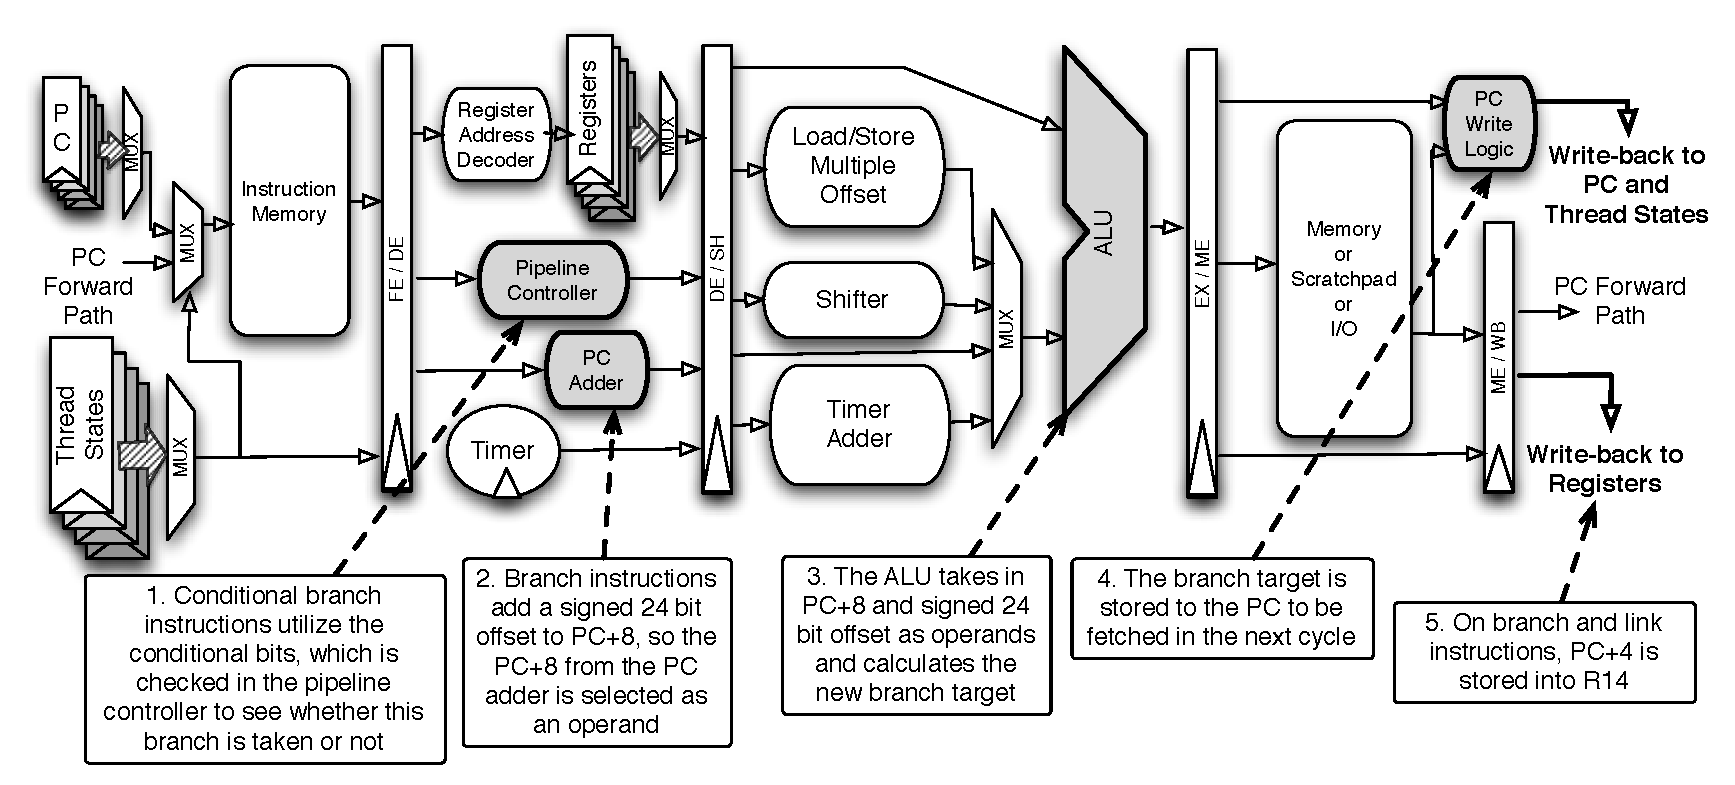
\includegraphics[scale=.54]{figs/branch_pipeline_implementation}
  \end{center}
  \vspace{-3mm}
  \caption{Branch Instruction Execution in the PTARM Pipeline}
  \label{fig:branch_pipeline_implementation}
\end{figure}

The branch instructions for the ARM ISA calculate the branch target address by adding a 24 bit signed offset, specified in the instruction, to the current PC incremented by 8. 
Thus, the PC+8 output from the PC Adder is used as an operand for the ALU to calulate the target branch address.  
Once the address is calculated, it is written back to its thread's next PC ready to be fetched. 
If the instruction is a branch and link ($bl$) instruction, PC+4 is propagated down the pipeline and written back to the link register (R14).   

All branch instructions, whether conditionally taken or not, all take only one thread cycle to execute.
But more importantly, the next instruction in the thread executed after the branch , whether it is a conditional branch or not, is not stalled or speculatively executed.
Rather, it is fetched after the conditional branch is resolved, and the branch target address is calculated. 
%The execution time of instructions from the same thread after the branch is not stalled nor affected by the branch instruction.  
The thread-interleaved pipeline simplifies the implementation of the branches and removes the need for control hazard handling logic.
Instead of speculating the branch target address the next processor cycle, instructions from other threads will be fetched and executed.

\subsection{Memory Instructions}
There are two type of memory instructions implemented in PTARM from the ARM ISA: Load/Store Register and Load/Store Multiple.
We discuss both type of memory instructions, and also present the special case when a load instruction loads to R15.
This triggers a branch which loads the branch target address from memory.  
Although this slightly complicates our pipeline design, we show that it does not affect the timing predictability and execution of the instruction, and subsequent instructions after the triggered branch.
Currently load/store halfword and doubleword are not implemented in PTARM, as they fall under the miscellaneous instructions category. 
These instructions can easily be implemented using the same principles described below.       
  
\subsubsection{Load/Store Register}
\label{sec:ptarm_instruction_ldstr}
Load instructions load data from memory to registers, and store instructions store data from registers to memory.
Store instructions utilizes the third register read port to read in the register value to be stored to memory.
The memory address is formed by combining a base register and an offset value.
The offset value can be a 12 bit immediate encoded from the instruction, or a register operand that can be shifted.
The current load/store instructions supports word or byte operations.
Figure~\ref{fig:ldstr_pipeline_implementation} describes how load/store register is implemented in the pipeline.

\begin{figure}[h]
  \begin{center}
    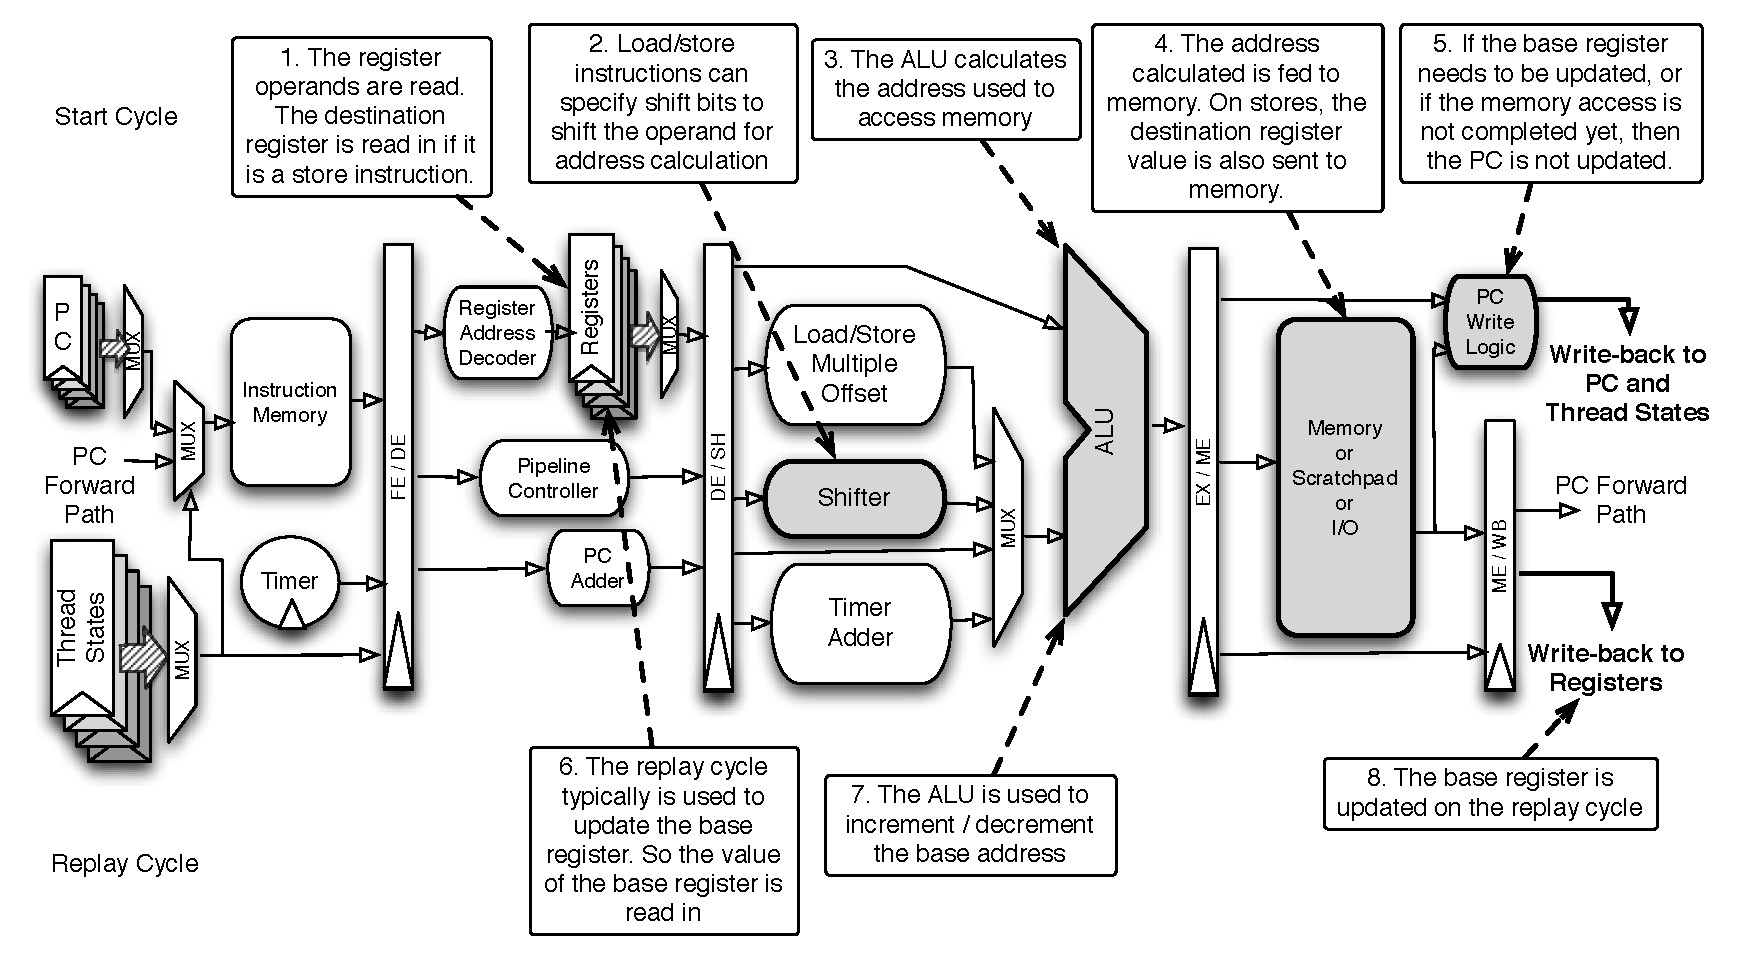
\includegraphics[scale=.54]{figs/ldstr_pipeline_implementation}
  \end{center}
  \vspace{-3mm}
  \caption{Load/Store Instruction Execution in the Ptarm Pipeline}
  \label{fig:ldstr_pipeline_implementation}
\end{figure}

Accesses to different memory regions yield different latencies for memory instructions.
When the memory address accesses the scratchpad or boot code memory region, memory operations are completed in a single processor cycle.
Thus, the data is ready in the following (\emph{writeback}) stage to be written back to the registers.
However, if the DRAM is accessed, the request must go through the DRAM memory controller, which takes either three or four thread cycles to complete.
Our thread-interleaved pipeline implementation does not dynamically switch threads in and out of execution when they are stalled waiting for memory access to complete. 
Thus, when a memory instruction is waiting for the DRAM, the same instruction is replayed by withholding the update for the next PC, until the data from DRAM arrives and is ready to be written back in the next stage.
The memory access latencies to the I/O region is device dependent.   
Currently, all I/O devices connected to PTARM all interface with PTARM through single cycle memory mapped control registers.
So memory instructions accessing I/O regions currently also take only one thread cycle.  

Load/store instructions in ARM have the ability to update the base register after any memory operation. 
This compacts code that reads arrays, as a load or store instruction can access memory and updates the base register so the next memory access is done on the updated base register.
The addressing mode of the instruction dictates how the base address register is updated. 
Pre-indexed addressing mode calculates the memory address by first using the value of the base register and offset, then updates the base register after the memory operation. 
Post-indexed addressing mode first updates the base register, then uses the updated base register value along with the offset to form the memory address.
Offset addressing mode simply calculates the address from the base register and offset, and does not update the base register. 
When pre and post-indexed addressing modes are used, load operations require an additional thread cycle to complete.
This results from the contention of the single write port in the register file. 
Because the register only has one write port, we cannot simultaneously write back a loaded result and update the base register in the same cycle.
Thus, an extra pass through the pipeline is required to resolve the contention and update the base register. 
%In the hardware implementation, for memory instructions that access the DRAM or I/O region, it is possible to update the base register earlier during the cycles where the instruction is waiting for access to complete.
%However, the current PTARM implementation uses the same logic and datapath for all memory accesses (scratchpad, DRAM, I/O etc) to minimize hardware resources, so an additional cycle is used to update the base register for all memory accesses regardless of the address region they are accessing.

\subsubsection{Load/Store Multiple}
The load/store multiple instruction is used to load (or store) a subset, or possibly all, of the general purpose registers from (or to) memory.
This instruction is often used to compact code that pushes (or pops) registers to (or from) the program stack.
The list of registers used is encoded in a 16 bit bit-vector as part of the instruction.
The 0th bit of the bit-vector represents R0 and the 15th bit represents R15.
A base register supplies the base memory address that is loaded from or stored to.
The base address is sequentially incremented or decremented by 4 bytes and used as the memory address for each register that is subsequently operated on. 
Figure~\ref{fig:ldstrm_pipeline_implementation} shows how the load/store multiple instruction executes in the pipeline. 

\begin{figure}[h]
  \vspace{-15pt}
  \begin{center}
    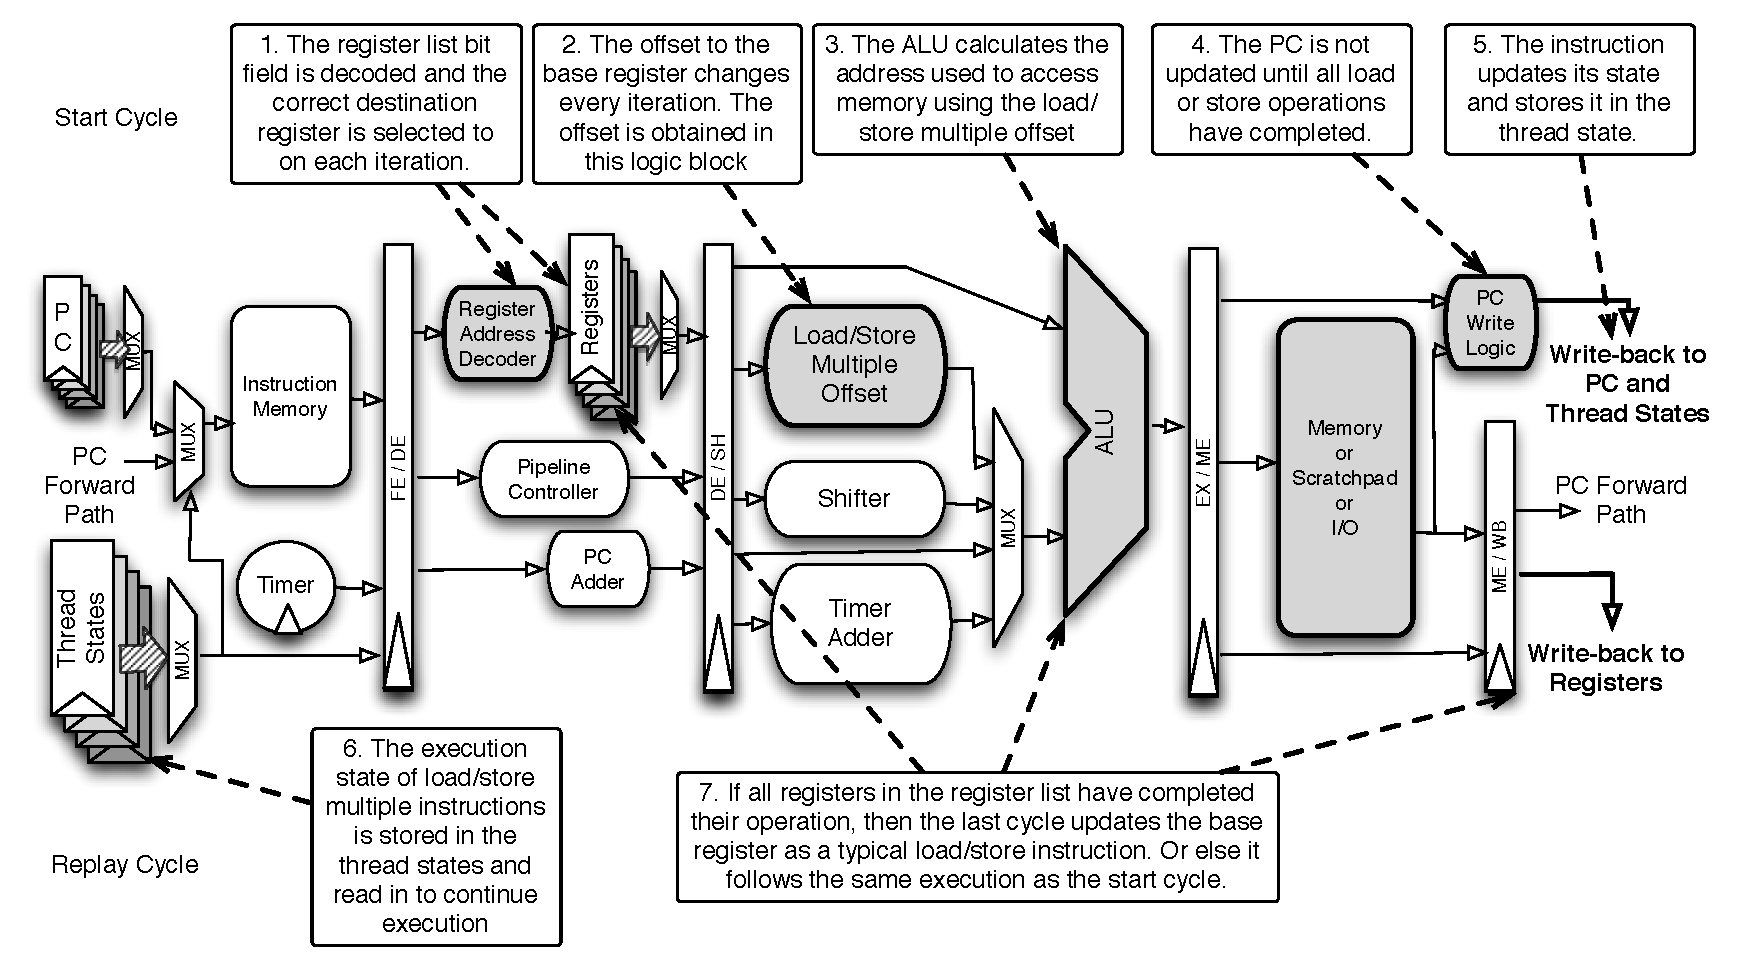
\includegraphics[scale=.54]{figs/ldstrm_pipeline_implementation}
  \end{center}
  \vspace{-3mm}
  \caption{Load/Store Multiple Instruction Execution in the PTARM Pipeline}
  \label{fig:ldstrm_pipeline_implementation}
\end{figure}

The load/store multiple instruction is inherently a multi-cycle instruction, because each thread cycle can only write back one value to the register or store one value to memory.
When the instruction is initially decoded, the register list is read and stored in the thread state keep track of the instruction progress.   
%The instruction state and remaining register list for load/store multiple instructions are stored in thread state during execution.
During each execution cycle, the \emph{register address decoder} in the pipeline decodes the register list and determines the register being operated on.
For loads, this indicates the destination register that is written back to.
For stores, this indicates the register whose value will be stored to memory.
The \emph{load/store multiple offset} block calculates the current memory address offset based on the remaining bits in the register list.
The offset is added to the base register to form the memory address fed into memory.
Each cycle, the register that is operated on is cleared from the remaining register list. 
The instruction completes execution when all registers have been operated on, which occurs when all bits in the register list are cleared. 

The execution time of this instruction depends on the number of registers specified in the register list and the memory region that is being accessed. 
For accesses to the scratchpad or boot code, each register load or store takes only a single cycle. 
However, if memory accesses are to the DRAM region, then each register load/store will take multiple cycles.
Load/store multiple instruction can also update the base register after all the register operations completes. 
Similar to the load/store register instruction, an additional thread cycle will be used to update the base register for load multiple instructions.
Although the execution time of this instruction seems to be dynamic depending on the number of registers specified in the register list, but this number can be determined statically from the instruction binary. 
Thus, the execution time of this instruction can easily be statically analyzed.   

\subsubsection{Load to PC}
\label{sec:load_to_pc}    
When a load instruction loads to R15, a branch is triggered in the pipeline.
This is also the case for load multiple instructions when bit 15 is set in the register list bit-vector.
In our five stage pipeline, the PC is updated in the memory stage to prepare for the next instruction fetch for the thread.   
However, if the branch target address is loaded from memory, the address is not yet present in the memory stage to be committed; only at the writeback stage will it be present. 
Thus, we introduce a forwarding path that forwards the PC straight from the writeback stage to instruction fetch if the next PC comes from memory. 
Figure~\ref{fig:ld_to_pc_pipeline_implementation} shows how this is implemented in our pipeline.   

\begin{figure}[h]
  \vspace{-15pt}
  \begin{center}
    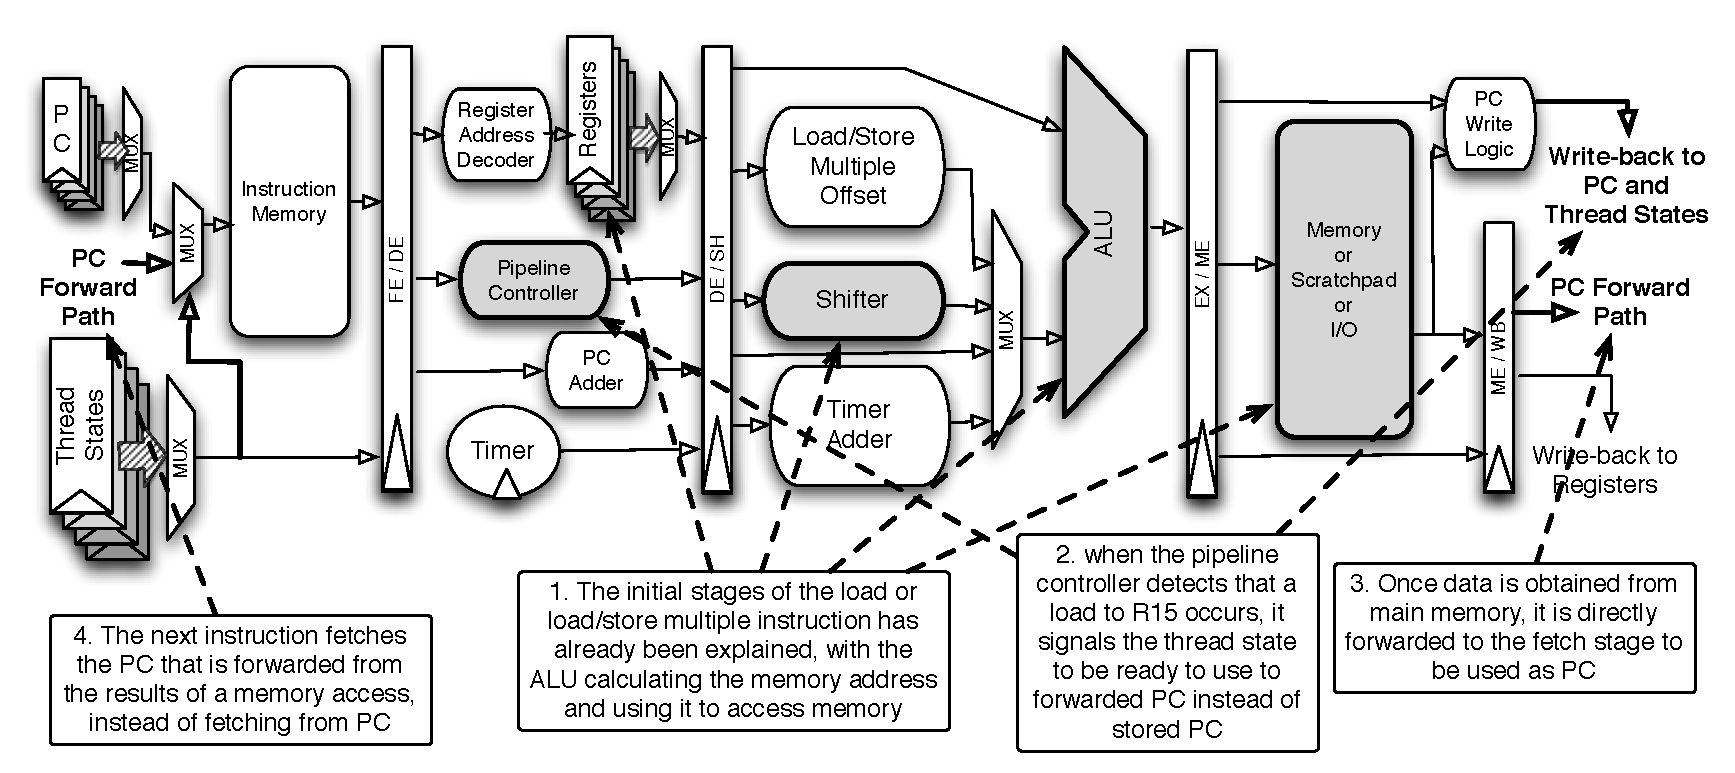
\includegraphics[scale=.54]{figs/ld_to_pc_pipeline_implementation}
  \end{center}
  \vspace{-3mm}
  \caption{Load to R15 Instruction Execution in the PTARM Pipeline}
  \label{fig:ld_to_pc_pipeline_implementation}
\end{figure}

An extra multiplexer is placed in the fetch stage before the instruction fetch to select the forward path.
When a load to R15 is detected, it will signal the thread state to use the forwarded PC on the next instruction fetch, instead of the one stored in next PC.
We showed in figure~\ref{fig:four_thread_pipeline} that for the same hardware thread, the fetch and writeback stage overlap in execution.  
As the memory load will be completed by the writeback stage, the correct branch target address will be selected and used in the fetch stage.

Section~\ref{sec:pipeline_hazards} discussed the timing implications of data-forwarding logic in the pipeline.
%Those same principles are applied in this situation.
Although it seems the selection of PC is dynamic, but when forwarding occurs is actually static; the PC forwarding only and always occur when instructions load from memory to R15.
This mechanism has no additional timing effects on any following instructions, as no stalls are needed to wait for the address to be ready. 
Even if the load to R15 instruction is accessing the DRAM region, the execution time of this instruction does not deviate from a load instruction destined for other registers.
Although the target address will not be known until after the DRAM access completes, a typical load instruction also waits until the DRAM access completes before the thread fetches the next instruction. 
So this extra forwarding mechanism does not cause load to R15 instructions to deviate from other load timing behaviors.

If the load to R15 instruction updates the base register, then the forwarding path is not needed and not used. 
The extra cycle used to update the base register will allow us to propagate the results from memory to update the PC in the memory stage.
This timing behavior conforms to a typical load instruction that updates its base register. 

\subsection{Timing Instructions}
\label{sec:timing_inst_implementation}
Section~\ref{sec:programming_models} presented the instruction extensions to the ARM ISA to bring timing semantics at the ISA level.
These instructions are added using the co-processor instruction slots in the ARM instruction space. 
In particular, the timing instructions are implemented using co-processor 13.
Table~\ref{table_deadline_insts} summarizes the instructions, their op codes, and their operations.
All instructions have the assembly syntax ``\textbf{\textit{cdp, p13, $<$opcode$>$ rd, rn, rm, 0}}'', with $<$opcode$>$ differentiating the instruction type.
   
\begin{table}[h]
\noindent\makebox[\textwidth]{%
\begin{smalltabular}{ | l | l | p{6cm} | }
  \hline                        
  Type & Opcode &  Functionality \\ \hline
  \textbf{\textit{get\_time}} & 8  & 
timestamp = \textit{current\_time}; \newline
crd = high32(timestamp); \newline
crd+1 = low64(timestamp); 
  \\ \hline 
  \textbf{\textit{delay\_until}} & 4 & 
deadline = (crm $<<$ 32) + crn; \newline
while ( \textit{current\_time} $<$ \textit{deadline} )  \newline
\hspace*{5 pt} stall\_thread(); 
 \\ \hline 
  \textbf{\textit{exception\_on\_expired}} & 2 &
offset = (crm $<<$ 32) + crn; \newline
register\_exception(offset);  
\\ \hline
  \textbf{\textit{deactivate\_exception}} & 3 &
deactivate\_exception();  
\\ \hline
\end{smalltabular}}
\vspace{1mm}
\caption{List of assembly deadline instructions}
\label{table_deadline_insts}
\end{table}

All timing instructions use the \emph{platform clock} to obtain and compare deadlines.
Instead of using an external timer that is accessed through the I/O bus, the \emph{platform clock} is implemented as a core hardware unit in the pipeline.  
The deterministic single cycle access latency to the clock value increases the precision of and predictability of timing operations on our processor.  
The \emph{platform clock} is implemented in the \emph{timer} hardware block shown in figure~\ref{fig:ptarm_pipeline_five_stage}.   
An unsigned 64 bit value represents time in nanoseconds, and resets at zero when PTARM is reset.
Unsigned 64 bits of nanoseconds covers approximately 584 years. 
The \emph{platform clock} is implemented with a simple 64 bit adder increments to the current time value each processor clock cycle. 
We clock PTARM at 100$MHz$, so the timer value is incremented by 10 nanoseconds every processor cycle.
If the processor clock speed is modified, then the timer increment must be modified to reflect the correct clock speed. 
For architectures that allow the processor frequency to be scaled, the \emph{platform clock} must also be adjusted when the frequency is scaled.  
For the purposes of clock synchronization, the time increment is stored in a programmable register that can adjust the timer increment to synchronize with external clocks. 
The timer increment value can only be modified through a privileged \emph{set\_time\_increment} instruction, to protect the programmer from accidentally speeding up or slowing down the \emph{platform clock}.

The timestamp associated with each instruction execution is latched during the fetch stage of the pipeline.
In order words, the \emph{time of execution} for each instruction is the precise moment when the instruction begins execution in the pipeline.
Timestamps are 64 bits, so they require two 32 bit registers to store.
The timestamps are loaded into general purpose registers with the \gettime\ instruction, so standard register-to-register instructions can be used to manipulate the timestamps. 
PTARM does not currently provide 64 bit arithmetic operations, so programmers must handle the arithmetic overflow in software.
The timing effects from the timing instructions are thread specific.   
Each thread operates on its own timestamps, and are not affected by the timing instructions from other threads.
With 4 hardware threads interleaved through the pipeline, each hardware thread observes the time change once every 4 processor clock cycles.
So the minimum observable interval of time for our implementation is $40 ns$. 
The timing implications of this is discussed in section~\ref{subsec:precision_timing_inst_ptarm}.
We now describe how the pipeline executes each timing instruction.  
	
\subsubsection{Get\_Time}    
The \gettime\ instruction is used to obtain the current clock value.
The timestamp obtained from \gettime\ represents the \emph{time of execution} of this instruction.
The execution of \gettime\ is straightforward and shown in figure~\ref{fig:get_time_pipeline_implementation}. 
\begin{figure}[h]
  \vspace{-15pt}
  \begin{center}
    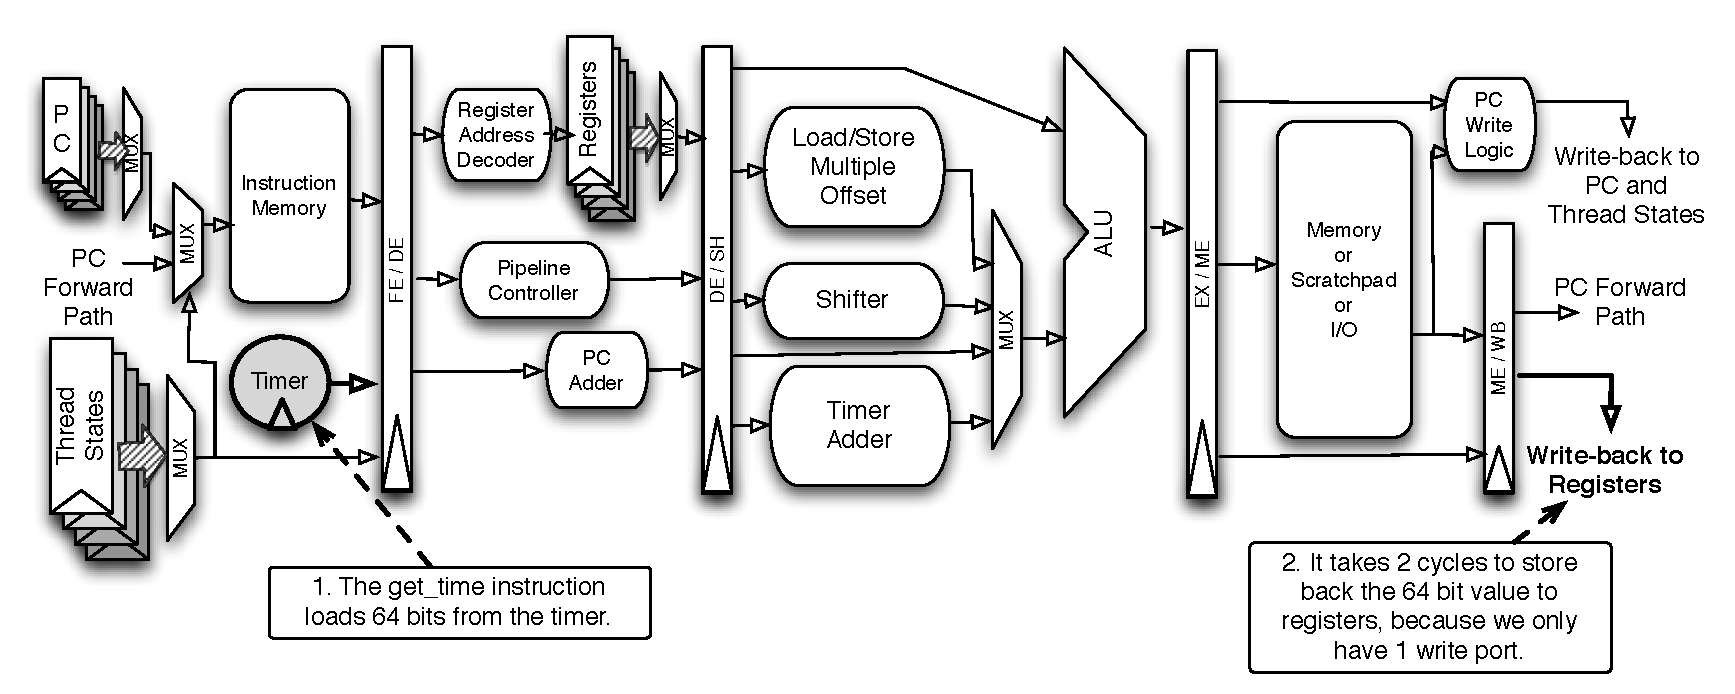
\includegraphics[scale=.54]{figs/get_time_pipeline_implementation}
  \end{center}
  \vspace{-3mm}
  \caption{Get\_Time Instruction Execution in the PTARM Pipeline}
  \label{fig:get_time_pipeline_implementation}
\end{figure}
The timestamp is latched during instruction fetch, and stored into registers.
Because the register file only contains one write port, so \gettime\ takes two thread cycles to complete; each cycle writes back 32 bits of the timestamp. 
The timestamp is written back to the destination register rd and rd+1, with rd storing the lower 32 bits and rd+1 storing the higher 32 bits. 
This instruction will not write to R15 (PC), and it will not cause a branch. 
If R14 or R15 is specified as rd, causing a potential write to R15, then this instruction will simply act as a NOP.

\subsubsection{Delay\_Until}    
\emph{Delay\_until} is used to delay the execution of a thread until the \emph{platform clock} exceeds an input timestamp.
It takes in 2 source operands that forms the 64 bit timestamp that is checked against the \emph{platform clock} every thread cycle.
As described in section~\ref{sec:programming_models}, the \emph{delay\_until} instruction can be used to specify a lower bound execution time for code blocks.
This could be useful for synchronization between tasks or communicating with external devices.
Figure~\ref{fig:delay_until_pipeline_implementation} shows the execution of the \emph{delay\_until} instruction in the PTARM pipeline.       
\begin{figure}[h]
  \vspace{-15pt}
  \begin{center}
    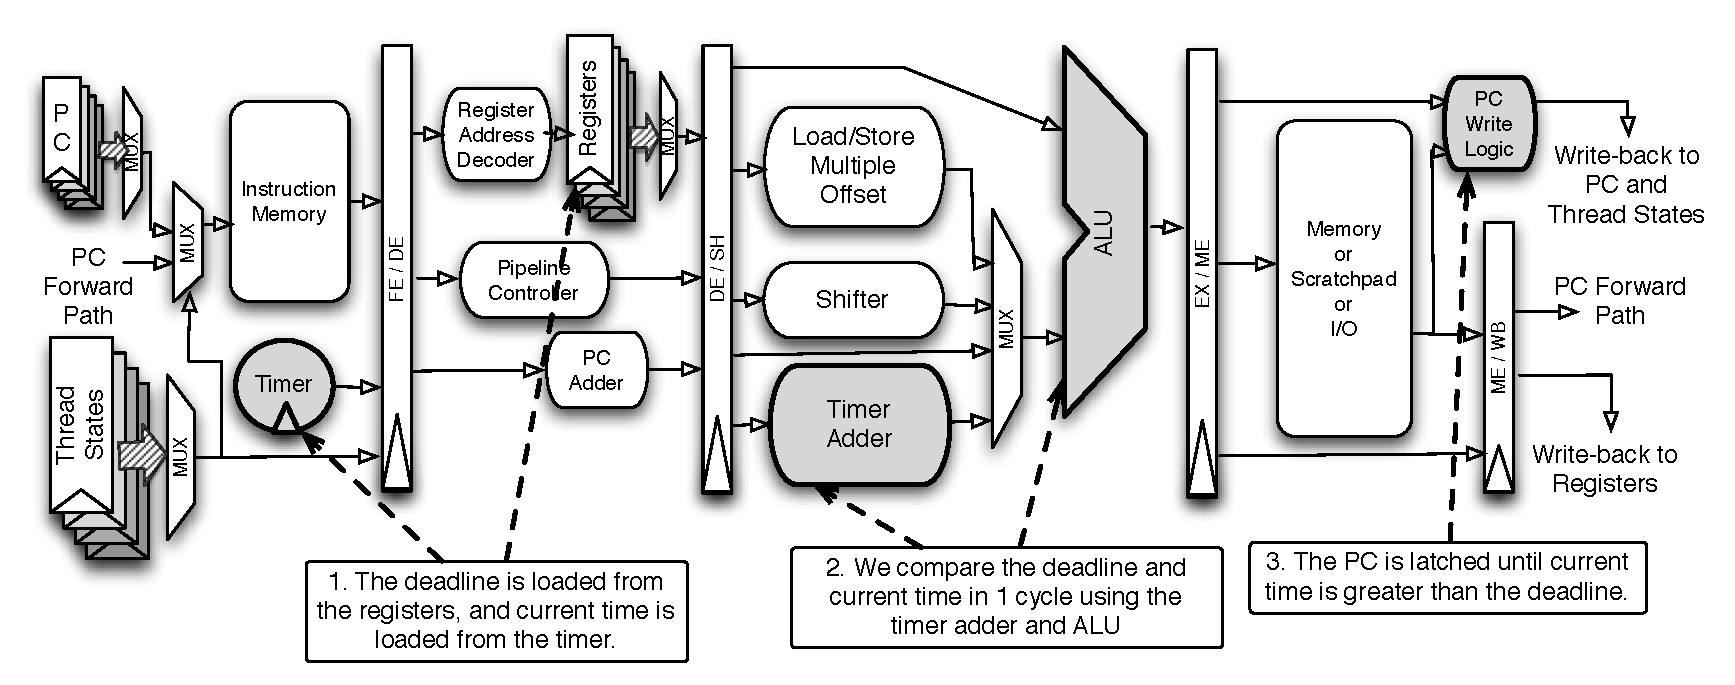
\includegraphics[scale=.54]{figs/delay_until_pipeline_implementation}
  \end{center}
  \vspace{-3mm}
  \caption{Delay\_Until Instruction Execution in the PTARM Pipeline}
  \label{fig:delay_until_pipeline_implementation}
\end{figure}

The \emph{delay\_until} instruction highlights the reason \emph{timer adder} is added into the pipeline.
During the execution of \delayuntil\, the clock value is used every thread cycle to be compared with the input timestamp.
However, the input timestamp and clock value are both 64 bit values.
Without the additional \emph{timer adder} in the pipeline, comparing 64 bits would require two thread cycles using our 32 bit ALU. 
This increases the jitter of this instruction by a factor of two, because now the two timestamps can only be compared every two thread cycles. 
The added \emph{timer adder} allows \emph{delay\_until} to compare the timestamps every thread cycle, and ensure that no additional threads cycles elapses after the input timestamp is reached. 
To delay program execution, the PC is only updated when the clock value is greater or equal to the input timestamp.
No thread states are modified by \delayuntil.
If the clock value already exceeds the input timestamp when the instruction is first decoded, then this instruction acts as a NOP. 
The PC is simply updated and the program execution continues.
We detail the jitter effects of \delayuntil\ in section~\ref{sec:jitter_of_timing_instructions}.

\subsubsection{Exception\_on\_Expire and Deactivate\_Exception}
\Delayuntil\ passively compares an input timestamp against the platform clock when the instruction is executed.
\emph{Exception\_on\_expire} registers a timestamp to be actively checked against the \emph{platform clock} in hardware.
When the \emph{platform clock} exceeds the registered timestamp value, a \timerexpired\ exception is thrown.
\emph{Deactivate\_exception} deactivates the timestamp that is actively being checked so no exception will be thrown.
The idea is similar to setting of timer interrupts on embedded platforms, which are typically controlled through memory mapped registers.

\begin{wrapfigure}{r}{0.4\textwidth}
  \vspace{-20pt}
  \begin{center}
    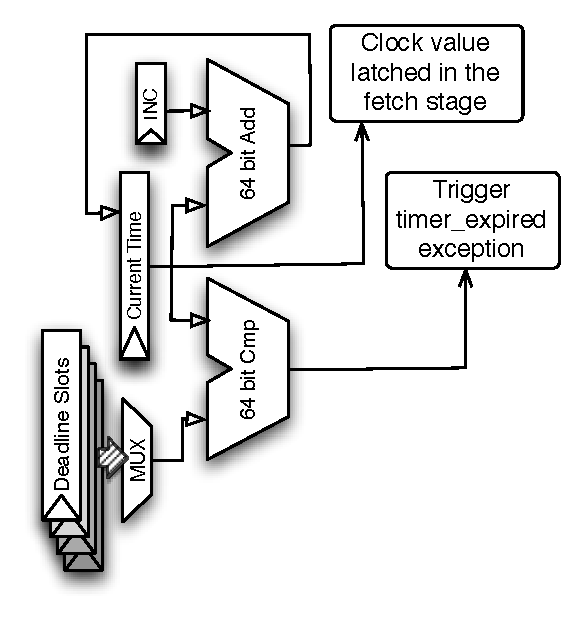
\includegraphics[scale=.6]{figs/timer_unit_circuit}
  \end{center}
  \vspace{-5mm}
  \caption{Implementation of Timer Unit}
  \label{fig:timer_unit_circuit}
  \vspace{-13pt}
\end{wrapfigure} 

Within the \emph{timer} unit, there is one 64 bit deadline slot for each thread to register a timestamp to be actively checked. 
PTARM has 4 hardware threads, so there are four deadline slots in the \emph{timer} unit. 
Whenever an \emph{exception\_on\_expire} instruction is executed, the two source operands form the timestamp that is stored to the thread's corresponding deadline slot.
The \exceptiononexpire\ instruction takes only one thread cycle to execute.
It simply stores and activates the timestamp in the thread's deadline slot.
Once activated, program execution continues, and the deadline slot timestamp is compared against the \emph{platform clock} every thread cycle in the \emph{timer} unit, until deactivated with \deactivateexception.
When the \platformclock\ is greater or equal to the stored timestamp, a \timerexpired\ exception is triggered by the \emph{timer} unit, and the deadline slot is deactivated to ensure only one exception is thrown per timestamp.
When \deactivateexception\ is executed, if the deadline slot for the thread is active, then it will be deactivated. 
If the deadline slot for the thread is non active, then \deactivateexception\ will do nothing.
The implementation of the \emph{timer} unit is shown in figure~\ref{fig:timer_unit_circuit}.   

\Exceptiononexpire\ and \deactivateexception\ instructions are thread specific; each thread has its own dedicated deadline slot.
The handling \timerexpired\ exceptions, described in section~\ref{subsec:exception_handling_in_ptarm}, preserves temporal isolation for the hardware threads in the pipeline.
So the timing effects of \exceptiononexpire\ and \deactivateexception\ can only affect the specific thread they are executed on.
The timing details and jitter introduced with this mechanism is detailed in section~\ref{sec:jitter_of_timing_instructions}.

Each thread currently can only check for one timestamp in hardware. 
To create the effects of multiple timestamps to being checked in hardware, the timestamps need to managed in software and share the one physical deadline slot.
It is possible to add more deadline slots for threads in the \emph{timer} unit at the cost of increased hardware usage.
One deadline slot for each thread (4 deadline slots total) requires a multiplexer and a 64 bit comparator against the current clock, as shown in figure~\ref{fig:timer_unit_circuit}.
So more deadline slots would add more comparators and multiplexers, plus an additional OR gate to OR the exception triggering signal. 
The instructions \exceptiononexpire\ and \deactivateexception\ can easily be modified to take an id representing a specific deadline slot.

\section{Implementations}
\subsection{PTARM VHDL Soft Core}
\label{sec:ptarm_vhdl_soft_core}
  
The PTARM soft core is written in VHDL.
It includes the pipeline, scratchpad memories, predictable memory controller and connects to several I/O devices on the FPGA.
These include several LEDS, the UART, DVI controller and the DDRII DRAM.
All I/O devices are connected through the I/O bus, while the DDRII DRAM is connected directly to the DRAM controller.
Figure~\ref{fig:ptarm_vhdl_high_level} shows the high level block diagram of the PTARM soft core.

\begin{wrapfigure}{r}{0.5\textwidth}
  \vspace{-20pt}
  \begin{center}
    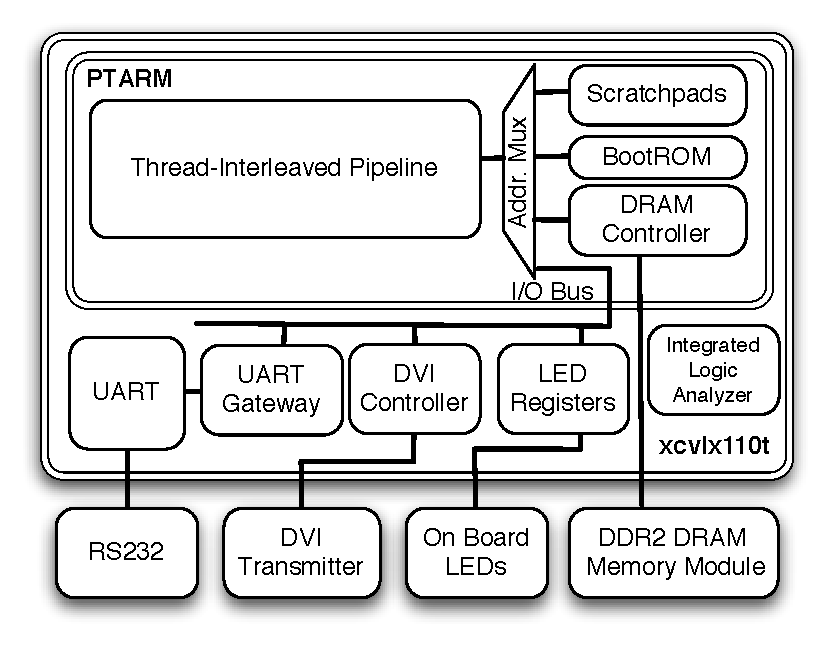
\includegraphics[scale=.6]{figs/ptarm_vhdl_high_level}
  \end{center}
  \vspace{-3mm}
  \caption{PTARM Block Level View}
  \label{fig:ptarm_vhdl_high_level}
  \vspace{-10pt}
\end{wrapfigure} 

The LEDs are memory mapped and can be toggled by setting and clearing bits.
PTARM communicates to the UART through the UART gateway, which queues read and write requests from the core and relays it to the UART.
The default buffer size on the UART gateway is one.
The UART gateway status registers are mapped to memory I/O locations so programs can poll them to determine that status of the UART.  
Currently all read and write operations to the UART is done through blocking procedure calls. 
The UART runs at a baud rate of 115200 and can send and receive bytes.

The DVI controller is used to control the DVI input port on the FPGA, so a monitor can be connected.
\todo{look at documentation of the DVI controller, what mode we're using it.}
We demo a DVI controller application similar to the one presented in~\cite{ip2006processor}, where a vga controller is managed purely in software through the deadline instructions presented in the paper.
Here, we use the timing constructs presented in section~\ref{sec:programming_models} to control the sending out of vertical and horizontal sync signals in software.
As one hardware thread manages the sync signals, other hardware threads in our core can be used to calculate and draw to the screen buffer.  
Because hardware threads are temporally isolated, the timing of hardware sync signals are not affected by the operations on other hardware threads.  

We synthesized the core on a Virtex-5 lx110t FPGA to obtain the maximum clock frequency and resource usage. 
\todo{show area and clock speed on FPGA}  
We current clock PTARM at $100MHz$ and the memory controller at $200MHz$. 
All VHDL source code, software code samples, and instruction manual can be downloaded from http://chess.eecs.berkeley.edu/pret.   

\subsection{PTARM Simulator}
\label{sec:ptarm_sim}
Along with the VHDL soft core, we also developed a C++ cycle accurate software simulator of our architecture.
The simulator is meant for architectural exploration, and provides better debugging for software written for PTARM.  
The C++ simulator models the pipeline and memory hierarchy, including the predictable DRAM controller.  

The simulator provides a framework that allows us to do more architectural exploration and observe the behavior.
For example, the DMA units for each thread mentioned in section~\ref{sec:ptarm_dram_integration} that 
provide threads with the ability to transfer contents from the DRAM to the scratchpads in the background is currently only implemented on the simulator. 
The simulator allows us to quickly test out different software behaviors and verify our assumptions. 
The simulator and corresponding documentation can be downloaded from http://chess.eecs.berkeley.edu/pret. 

\todo{present benchmark numbers on the simulator and compare to others}

\section{Timing Analysis}
\label{sec:wcet}
\label{subsec:precision_timing_inst_ptarm}

%mention that a full scaled worst case execution time analysis is beyond the scope of this thesis.
%but do a brief summary on how it's done, cite wilhelm's group's research summary
Worst-case execution time (WCET) analysis is a combined analysis of the control paths that the software might exhibit, and the time it takes to execute those paths on the underlying architecture. 
A plethora of research has been done on the software analysis of control paths. 
Wilhelm et al.~\cite{wilhelm-survey-paper} presented a survey of tools and techniques available for worst-case path enumeration and loop analysis etc.
However, the precision of the WCET analysis of those techniques ultimately depend on the underlying architecture implementation~\cite{Heckmann2003processor}.
Architectures that exhibit wildly unpredictable execution times will result in overly conservative WCET analysis, even if the software structure is simple. 
Designed as a predictable architecture, the instructions of PTARM all exhibit deterministic timing behaviors, allowing a more precise WCET as software analysis progresses. 
In section~\ref{sec:ptarm_instructions} we discussed the implementation of each instruction and explained the execution time of each instruction type.
Table~\ref{table:ptarm_instruction_timing} summarizes the execution time each instruction takes in terms of \emph{thread cycles}. 

\begin{table}[h]
\noindent\makebox[\textwidth]{%
\begin{smalltabular}{ | p{4cm} | c || p{9cm} | }
  \hline                        
  \textbf{Instruction Type} & \textbf{Thread Cycles} & \textbf{Notes}    \\ \hline
  Data Processing  & 1 & \multirow{2}{9cm}{ ${\ast}$: an additional cycle is added if pre or post-index offset is used in the address mode.}  \\ \cline{1-2} 
  Branch  & 1 &  \\ \cline{1-2}
  Load/Store (SPM)  & 1$^{\ast}$ &  \multirow{4}{9cm}{ ${\phi}$: the dram latency is 3 or 4 thread cycles depending on the alignment of the pipeline and the dram controller backend, as described in section~\ref{sec:ptarm_dram_integration}. For conservative estimates, 4 thread cycles is used. } \\ \cline{1-2} 
  Load/Store (BootROM)  & 1$^{\ast}$ & \\ \cline{1-2}  
  Load/Store (DRAM) & 4$^{\phi \dagger \ast}$ & \\ \cline{1-2}
  Load/Store Multiple & $N_{reg} \times L_{mem}$ $^{\Delta \ast}$ &  \\  \cline{1-2}
  Software Interrupt (SWI) & 1 & \multirow{4}{9cm}{ ${\dagger}$: a single store buffer is implemented, as described in section~\ref{sec:ptarm_dram_store_buffer}, so non-consecutive stores take only 1 thread cycle, while consecutive stores require the full dram latency of 3 or 4.}\\    \cline{1-2}
  get\_time  & 2 &  \\ \cline{1-2}
  delay\_until  & 1 $^{\sigma}$ & \\    \cline{1-2}
  exception\_on\_expire  & 1  &    \\   \cline{1-2}
  deactivate\_exception & 1 &  \multirow{2}{9cm}{ ${\Delta}$: $N_{reg}$ is number of registers specified in the instruction. $L_{mem}$ is the latency of the memory region operated on.} \\  \cline{1-2}
  \multicolumn{2}{|c|}{} &  \\ \cline{1-2}
  \multicolumn{2}{|c|}{} &   \multirow{2}{9cm}{${\sigma}$: denotes the minimum execution time. Actual execution time depends on the system clock and the specified deadline.} \\ \cline{1-2}
  \multicolumn{2}{|c|}{} &\\ \hline
\end{smalltabular}}
\caption{Timing properties of PTARM instructions \todo{change this table}}
\label{table:ptarm_instruction_timing}
\end{table}

A \emph{Thread cycle} is the unit used to represent execution time on each thread.  
Timing analysis can be done separately for each hardware thread running on PTARM because the threads are temporally isolated; the execution time of each thread cannot be affected by other threads.
The thread-interleaved pipeline switches thread contexts every processor cycle in a predictable round robin fashion. 
Thus, each thread is fetched and executed in the pipeline every $N$ processor cycles, $N$ being the number of threads in the pipeline.
One \emph{Thread cycle} represents each time the thread enters in the pipeline, which is the thread's perceived notion of cycles.
The execution frequency of each thread ($F_{thread}$) is $F_{thread} = F_{processor}/N$, so each \emph{thread cycle} is $1/F_{thread}$ long. 
For example, our PTARM core is clocked at 100$MHz$ ($F_{processor} = 100 * 10^6$) and has 4 threads ($N=4$) , so each thread cycle is $1/((100 * 10^6)/4) = 40 * 10^{-9}$ secs, or 40 nanoseconds long.
The length of the \emph{thread cycle} will not change because of the predictable thread-switching policy, making it a reliable unit of measurement for execution time.   


\subsection{Memory instructions}
Data-processing instructions typically have straightforward execution times on most architectures.
In our case, branch instructions also have very a predictable and straightforward execution, as the branch penalty is completely hidden within the thread interleaving.
The memory instructions in our architecture however can have several different latencies depending on addressing mode or region of access, as listed in table~\ref{table:ptarm_instruction_timing}.
For memory instructions that use pre or post-indexed addressing mode to update the base register, an additional cycle latency is needed to write back to the base register, as described in the instruction implementation in section~\ref{sec:ptarm_instruction_ldstr}.
But the addressing mode of load/store instructions can be determined statically, as it is part of the instruction encoding, so it does not affect the complexity or precision of execution time analysis. 

For load instructions, the exposed memory hierarchy allows us to clearly label and identify access latencies to different memory regions.
In execution time analysis, value analysis attempts to determine what memory addresses are accessed.     
In systems that use caches and hide the memory hierarchy, additional modeling of the cache state is still needed after the value analysis determines the potential memory addresses that are accessed.
However, with an exposed memory hierarchy with scratchpads, the precision of execution time analysis depends only on the value analysis. 
As soon as the memory address is determined, we can give a associate a precise memory access latency.
The worst-case DRAM latency of 4 thread cycles is derived from~\cite{ReinekeLiuPatelKimLee11_PRETDRAMControllerBankPrivatizationForPredictability}. 
This allows not only for a simpler timing analysis, but also a more accurate analysis.

For store instructions, the single store buffer as described in section~\ref{sec:ptarm_dram_store_buffer} can possibly hide the latency of store instructions if no other memory access instruction comes after it. 
Otherwise the store instruction will take the full memory access latency, depending on the memory access region of the store.
Timing analysis tools can mostly account for the store buffer by statically checking a few instructions ahead of the store instruction to see if there are memory accessing instructions.
The window of instructions that need to be checked is very narrow, so it should not really complicate the analysis.
If this is not possible, then conservatively, the full memory access latency should be used for each store, depending on the access region.

The execution time of load/store multiple instructions depend on the number of registers operated on, and the memory region it accesses. 
Because the register list is statically encoded in the instruction, the number of registers operated on can easily be statically determined.
Store multiple instructions do not benefit from the store buffer, so all accesses take the full memory access latency.
For each register that is operated on, the latency will depend on which memory region it accesses. 
The total execution time of the instruction will be the sum of the latencies for all register operations. 
If pre or post-indexed addressing mode is used, an extra cycle is added to update the base register, just as regular load/store instructions. 

\subsection{Timing instructions}
Even though the execution time of most timing instructions can be statically determined, they impact the execution time of the program in a very dynamic way.
For example, the execution of \exceptiononexpire\ and \deactivateexception\ only take one cycle, but when the \timerexpired\ exception is thrown, the execution time of the whole program is affected. 
To understand the timing effects of the timing instructions, we must understand the implementation effects on the precision of the timing instructions.
It is impossible for any hardware implementation to provide absolute precision of time, as we are limited by the precision of the digital synchronous circuits that discretize the notion of time. 
Although the timing extensions allow the manipulation of nanoseconds in software, with the thread-interleaved pipeline, the basic unit of time for each thread is one thread cycle, or 40 nanoseconds, in PTARM.
As a result, 40 nanoseconds is the shortest interval of time that is observable by each thread.
This can also be explained from the implementation of the pipeline.
Each thread only latches the timer value in the fetch stage, and the timestamp is propagated along the pipeline and associated with the instruction. 
Since there are four threads cycling in a round robin fashion, each thread latches the timer value only once every 4 processor cycles. 
With 100MHz clocking the pipeline in our implementation, 4 processor cycles is  equivalent to 40 nanoseconds. 

When setting deadlines, the execution time of the timing instructions must be taken into account. 
As explained in the implementation, each timing instruction latches the current platform time in the fetch stage.
That timestamp is used throughout instruction execution and associated as the current time.  
For example, the time value in the timestamp obtained from \gettime\ will contain the time before the execution of \gettime.
Since \gettime\ takes 2 thread cycles every execution, 80 nanoseconds will have elapsed when the timestamp is obtained from \gettime.
In the same way, \delayuntil\ latches the current platform time at the fetch stage each thread cycle, and compares with the input timestamp. 
\Delayuntil\ will delay program execution until the latched platform time is \emph{greater than or equal to} the input timestamp value.
So when \delayuntil\ completes its execution, the current platform time will be \emph{at least} 40 nanoseconds greater than the input timestamp specified, to account for the execution of \delayuntil. 

\begin{figure}[h]
  \begin{center}
    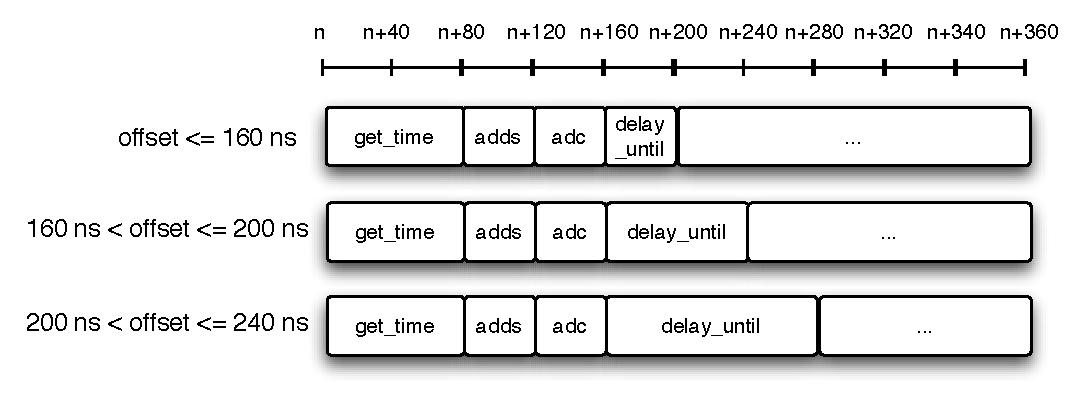
\includegraphics[scale=.7]{figs/delay_until_details}
  \end{center}
  \vspace{-3mm}
  \caption{Timing details of get\_time and delay\_until}
  \label{fig:delay_until_details}
\end{figure}

\todo{make figure for exception on expire!}

Figure~\ref{fig:delay_until_details} illustrates this effect by showing a timeline of execution for one thread on PTARM. 
The code segment starts executing at time $n$. 
The code only consists of \gettime, \delayuntil, and 2 add instructions used to add an offset to the timestamp obtained by \gettime.
For all 3 cases, the timestamp obtained by \gettime\ would contain the value $n$, even though the instruction after \gettime\ executes at $n+80$.
Taking into account the 2 thread cycles used to add the offset to the timestamp, if the offset is $\leq 160$, then the \delayuntil\ will simply serve as a NOP. 
This is because when \delayuntil\ is executed, it will latch $n+160$ for the platform time, and it will only delay program execution if the input timestamp is $> n+160$.
This is shown in the top case of the figure.
Notice that the instruction after \delayuntil\ executes at time $n+200$, which accounts for the 1 thread cycle it takes to execute \delayuntil.
Assuming \delayuntil\ does delay the program, in the worst-case, the instruction after \delayuntil\ executes $79 ns$ after the input timestamp. 
This can be observed if the offset is set to 161, which will result in the middle timeline shown in figure~\ref{fig:delay_until_details}.  
\Delayuntil\ will first latch the time $n+160$ to compare with the input timestamp of $n+161$. 
Because current platform time is less than input timestamp, \delayuntil\ will delay the execution of the program until the next cycle, when $n+200$ is latched to be checked against the input timestamp. 
At that point, \delayuntil\ will complete its execution, and the next instruction will execute at $n+240$.
This jitter results from the minimum observable time interval of $40 ns$ for each thread, causing \delayuntil\ to have an observable jitter of up to $40 ns$. 
\subsection{Timed Loop revisited}
\label{sec:timed_loop_revisited}
We give a concrete example of analysis of timing instructions on PTARM by deriving the \emph{offset} from the self compensating timed loop shown in section~\ref{sec:timed_loops}.
This timed loop detects whether the previous loop iteration missed its deadline. 
If it did, then the current iteration will execute a shorter version of the task in attempt to make up for the lost time, as shown in figure~\ref{fig:self_compensating_loop_timing}.  
\begin{figure}[h]
  \vspace{-3mm}
  \begin{center}
    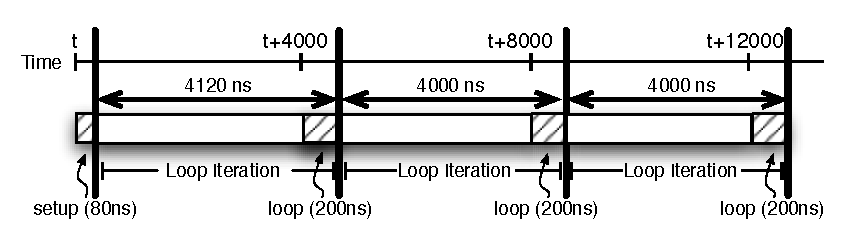
\includegraphics[scale=.7]{figs/self_compensating_loop_timing}
  \end{center}
  \vspace{-3mm}
  \caption{Execution of the self compensating timed loop}
  \label{fig:self_compensating_loop_timing}
\end{figure}
\vspace{-8mm}
\begin{lstlisting}[float=h, label=lst:timed_loop_compensate_revisit,caption=Timed loops with compensation revisited]
  cdp p13, 8, c2, c0, c0, 0  ; get_time, deadline timestamp stored in [c2, c3]
loop:
  cdp p13, 8, c4, c0, c0, 0  ; get_time, current timestamp stored in [c4, c5]
  subs r5, r5, #80           ; compensate for loop overhead and delay_until 
  sbc  r4, r4, #0            ; 

  subs r3, r3, r5            ; Check if previous iteration deadline is missed
  sbc  r2, r2, r4            ; 

  blmi task_short            ; execute shorter task if previous deadline mess 
  blpl task_normal           ; or else execute normal task 
  
  adds r3, r3, #4000         ; assuming the deadline is 4 us (4000 ns)
  adc r2, r2, #0             ; calculate the deadline timestamp for this iter.
  cdp p13, 4, c2, c2, c3, 0  ; delay_until
   
  b loop
\end{lstlisting}

\subsubsection{Obtaining the offset}

\begin{table}
\vspace{-5mm}
\begin{center}
\noindent\makebox[\textwidth]{%
\begin{smalltabular}{ | l | l | l r | }
  \hline
  \textbf{Time} & \textbf{TC} & \textbf{Instruction} & \textbf{Comment}\\ \hline \hline 
  t ns & n &  \textit{cdp p13, 8, c2, c0, c0, 0} & get\_time (deadline: t) \\  \hline
  \multicolumn{4}{|c|}{ -- -- Loop 1st iteration / No deadline miss -- -- } \\ \hline    
  t+80 ns & n+2 &  \textit{cdp p13, 8, c4, c0, c0, 0 } & get\_time, (current: t+80) \\
  t+160 ns & n+4 &  \textit{subs r5, r5, \#80} & (current -= 80)\\
  t+200 ns & n+5 &  \textit{sbc  r2, r2, r4} & (current: t)\\  
  t+240 ns & n+6 &  \textit{subs r3, r3, r5} & compare deadline (t) and current (t) \\
  t+280 ns & n+7 &  \textit{sbc  r2, r2, r4} & result is 0, clear cc[``n''] \\
  t+320 ns & n+8 &  \textit{blmi task\_short} & nop since cc[``n''] == 0\\
  t+360 ns & n+9 &   \textit{blpl task\_normal} & branch since cc[``n"] == 0\\  
    - ns & - &  \ldots & executing task\_normal \\  
  t+3800 ns & n+95 & \textit{adds r3, r3, \#4000} &  (deadline += 4000) \\
  t+3840 ns & n+96 & \textit{adc r2, r2, \#0} &  (deadline: t+4000) \\ 
  t+3880 ns & n+97 &  \textit{cdp p13, 4, c2, c2, c3, 0} & delay\_until, input timestamp is t+4000\\
  - ns & - & \ldots & delay\_until for 3 thread cycles\\  
  t+4040 ns & n+101 &  \textit{b loop} & jump back to loop \\ \hline
  \multicolumn{4}{|c|}{ -- -- Loop 2nd iteration / Deadline miss -- -- } \\ \hline    
  t+4080 ns & n+102 &  \textit{cdp p13, 8, c4, c0, c0, 0 } & get\_time, (current: t+4080)\\
  t+4160 ns & n+104 &  \textit{subs r5, r5, \#80} & (current -= 80)\\
  t+4200 ns & n+105 &  \textit{sbc  r2, r2, r4} & (current: t+4000)\\  
  t+4240 ns & n+106 &  \textit{subs r3, r3, r5} & compare deadline (t+4000) and current (t+4000)\\
  t+4280 ns & n+107 &  \textit{sbc  r2, r2, r4} & result is 0, clear cc[``n''] \\
  t+4320 ns & n+108 &  \textit{blmi task\_short} & nop since cc[``n''] == 0\\
  t+4360 ns & n+109 &   \textit{blpl task\_normal} & branch since cc[``n"] == 0\\  
  - ns & - &  \ldots & code for task\_normal \\  
  t+7960 ns & n+199 & \textit{adds r3, r3, \#4000} & (deadline += 4000) \\
  t+8000 ns & n+200 & \textit{adc r2, r2, \#0} & (deadline: t+8000) \\ 
  t+8040 ns & n+201 &  \textit{cdp p13, 4, c2, c2, c3, 0} & delay\_until, *no delay*\\
  t+8080 ns & n+202 &  \textit{b loop} & jump back to loop \\ \hline
  \multicolumn{4}{|c|}{ -- -- Loop 3rd iteration / Compensate with shorter task -- -- } \\ \hline    
  t+8120 ns & n+203 &  \textit{cdp p13, 8, c4, c0, c0, 0 } & get\_time, (current: t+8120)\\
  t+8200 ns & n+205 &  \textit{subs r3, r3, r5} & (current -= 80)\\
  t+8240 ns & n+206 &  \textit{sbc  r2, r2, r4} & (current: t+8040) \\
  t+8280 ns & n+207 &  \textit{subs r3, r3, r5} & compare deadline (t+8000) and current (t+8040)\\
  t+8320 ns & n+208 &  \textit{sbc  r2, r2, r4} & result is -40, set cc[``n''] \\
  t+8360 ns & n+209 &  \textit{blmi task\_short} & branch since cc[``n"] == 1 \\
  - ns & - &  \ldots & code for task\_short \\  
  t+10280 ns & n+257 &   \textit{blpl task\_normal} & nop since cc[``n''] == 1\\    
  t+10320 ns & n+258 & \textit{adds r3, r3, \#4000} & (deadline += 4000) \\
  t+10360 ns & n+259 & \textit{adc r2, r2, \#0} & (deadline: t+12000) \\ 
  t+10400 ns & n+260 &  \textit{cdp p13, 4, c2, c2, c3, 0} & delay\_until\\
  - ns & - &  \ldots & delay until time is t+12000 \\  
  t+12040 ns & n+301 &  \textit{b loop} & jump back to loop \\ \hline
   \multicolumn{4}{|c|}{ -- -- Loop 4th iteration / Execute normal task -- -- } \\ \hline    
  t+12080 ns & n+302 &  \textit{cdp p13, 8, c4, c0, c0, 0 } & get\_time, (current: t+12080)\\
  t+12160 ns & n+304 &  \textit{subs r3, r3, r5} & (current -= 80)\\
  t+12200 ns & n+305 &  \textit{sbc  r2, r2, r4} & (current: t+12000) \\
  t+12240 ns & n+306 &  \textit{subs r3, r3, r5} & compare deadline (t+12000) and current (t+12000)\\
  t+12280 ns & n+307 &  \textit{sbc  r2, r2, r4} & result is 0, clear cc[``n''] \\
  \hline 
\end{smalltabular}}
\end{center}
\vspace{-3mm}
\caption{Instruction execution trace of the self compensating timed loop\\ (TC = thread cycles)}
\label{table:timed-loop-compensate-timing}
\end{table}

\todo{state that we assume instruction is compiled to instruction scratchpad}
Listing~\ref{lst:timed_loop_compensate_revisit} shows the source code that is used to construct this timed loop. 
During the miss detection (lines 3 to 8), an additional \textit{offset} is used to compensate for the execution of \delayuntil\ and loop overhead.
Time elapses between the \delayuntil\ of the previous loop iteration (line 15), where the previous deadline timestamp is checked, and the \gettime\ used for miss detection (line 3) in the current iteration.
Without the offset compensation, the loop overhead will cause the miss detection to always detect a missed deadline.
This can be observed from table~\ref{table:timed-loop-compensate-timing}, where we show a sample execution trace of four iterations in this timed loop.  
Figure~\ref{fig:self_compensating_loop_timing} shows the timing behavior of these four iterations, where a missed deadline in the second iteration will cause the third iteration to compensate by executing the shorter version of the task.



In table~\ref{table:timed-loop-compensate-timing}, execution starts at time $t$.
As mentioned before, each thread cycle is $40ns$, which is reflect in the left most column that shows the progression of time.
We also show the thread cycle (TC) count, which starts at $n$ when execution begins.
The execution time of each instruction is according to table~\ref{table:ptarm_instruction_timing}.
In this code segment, we keep track of two timestamps each iteration. 
The \emph{deadline\_timestamp} keeps track of the loop deadlines, and is stored in registers r2 and r3.  
The \emph{current\_timestamp} is updated with \gettime\ in the beginning of each loop iteration to detect if the previous iteration missed its deadline.
It is stored in registers r4 and r5. 
The loop period is set to be $4 \mu s$, which is $4000 ns$ (100 thread cycles).
We add the loop period to the \emph{deadline\_timestamp} each loop iteration (lines 13 and 14 in the listing).  

\newcommand{\currentt}{\emph{current\_timestamp}}
\newcommand{\deadlinet}{\emph{deadline\_timestamp}}


The need for the \emph{offset} can be observed at the beginning of the second loop iteration.
At time $t+4080ns$, \gettime\ is called to initiate the miss detection sequence.
The previous \deadlinet\ is $t+4000$, which was met in the first iteration.  
However, \gettime\ updates the \currentt\ to $t+4080$, because the execution of \delayuntil\ and \emph{b loop} took 2 thread cycles combined. 
Thus, our miss detection accounts for this by subtracting the 2 thread cycles ($80ns$) overhead from \currentt\ before comparing it with \deadlinet.
In general, the overhead that needs to be account for is the time elapsed between the deadline checking \delayuntil\ instruction and the miss detection \gettime\ instruction.
Intuitively this is because we want to check whether the previous \delayuntil\ executed before the previous \deadlinet, so the \emph{offset} is used to calculate the time of execution of the previous \delayuntil.  

\subsubsection{Overhead of the self compensating timed loop}
In this self compensating timed loop, the loop period is set to $4000ns$, and regulated with the \delayuntil\ instruction.
However, the loop period includes the execution of the actual task along with the loop and timing control overhead.
The loop overhead in this example is only the branch instruction on line 17 in listing~\ref{lst:timed_loop_compensate_revisit}, which is 1 thread cycles (40 ns).
The overhead for timing control and self compensation consists of all the timing instructions, the arithmetic on the timestamps, and the 2 conditional branch instructions that determines which task to execute.
From table~\ref{table:timed-loop-compensate-timing} we can count a total overhead of 11 thread cycles including 1 \gettime\ (2 thread cycles), 1 \delayuntil\ (1 thread cycle), 6 arithmetic operations on the timestamps (6 thread cycles), and 2 conditional branch instructions (2 thread cycles).
Overall the timed loop contains an overhead of 12 thread cycles ($480ns$) , which means the executed tasks (both normal and short) have a timing requirement of 88 thread cycles ($3520ns$) in order for each loop iteration to meet its deadline.  
In the second loop iteration for our example, \emph{task\_normal} executed for 89 thread cycles, exactly one thread cycle over its timing requirement. 
As a result, the \delayuntil\ of the second loop iteration did not delay program execution, and the third iteration miss detection detects a missed deadline, and switches to execute \emph{task\_short}. 

\subsubsection{First loop iteration jitter}
The \emph{offset} previously derived is an overhead that is executed in every iteration of the loop.
In our code, the overhead only included the execution time of the \delayuntil\ and a branch, as we always unconditionally branch to the beginning of the loop. 
However, if the overhead was larger, for example, in a conditional loop structure, then it could introduce jitter for the first iteration.
An example is shown in figure~\ref{fig:setup_look_timing}, where we used an overhead of 200ns, instead of 80ns.
\begin{figure}[h]
  \vspace{-3mm}
  \begin{center}
    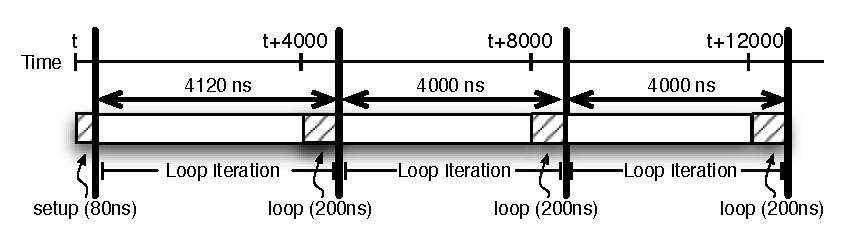
\includegraphics[scale=.9]{figs/setup_loop_timing}
  \end{center}
  \vspace{-3mm}
  \caption{Jitter caused by initial timed loop setup}
  \label{fig:setup_look_timing}
\end{figure}
We assume that the setup code remains the same with only one \gettime, and the \emph{offset} is adjusted to 200ns for the miss detection.
We also assume that the loop periond remains the same, 4000ns, and all loop iterations meet the loop period timing requirements. 
In this example, we see that the first iteration executes for 120ns longer than subsequent iterations.
The jitter for the first iteration is introduced by the execution time difference between the \emph{offset} and the setup code.  
Between the \delayuntil\ instructions, exactly 4000 ns elapses, because 4000 ns is added to the \deadlinet\ each loop iteration.   
The execution of the overhead is included within the 4000 ns, except for the first iteration. 
Instead, between the initial \deadlinet\ and the first \delayuntil, the only overhead that is observed is the execution of a \gettime\ instruction, which is 80 ns. 
Thus, the first iteration of the loop executes for an addition 120ns, which is the difference between the \emph{offset} and the execution time of the loop setup code.
This effect was not observed by the previous example because the \emph{offset} and the loop setup both took 80 ns.
As a result, for the previous example, each loop iteration takes exactly 4000 ns if all loop deadlines were met.   

\begin{lstlisting}[float=h, label=lst:timed_loop_compensate_adj,caption=Jitter adjusted timed loop ]
  mov r6, #0                 ; i = 0;
  mov r7, #0                 ; j = 0;
  
  cdp p13, 8, c2, c0, c0, 0  ; get_time, deadline timestamp stored in [c2, c3]
  subs r3, r3, #40           ; adjustment for first loop period 
  sbc  r2, r2, #0            ; deadline -= 40
loop:
  cdp p13, 8, c4, c0, c0, 0  ; get_time, current timestamp stored in [c4, c5]
  subs r5, r5, #200          ; compensate for loop overhead and delay_until 
  sbc  r4, r4, #0            ; 

  subs r3, r3, r5            ; Check if previous iteration deadline is missed
  sbc  r2, r2, r4            ; 

  blmi task_short            ; execute shorter task if previous deadline mess 
  blpl task_normal           ; or else execute normal task 
  
  adds r3, r3, #4000         ; assuming the deadline is 4 us (4000 ns)
  adc r2, r2, #0             ; calculate the deadline timestamp for this iter.
  cdp p13, 4, c2, c2, c3, 0  ; delay_until
	
  add r6, r6, #1             ; i += 1    
  add r7, r7, r6 LSL #1      ; j += i*2  
  cmp r7, #1000              ; 
  blt loop                   ; branch back if ( j < 10000 )
\end{lstlisting} 

\begin{figure}[h]
  \vspace{-3mm}
  \begin{center}
    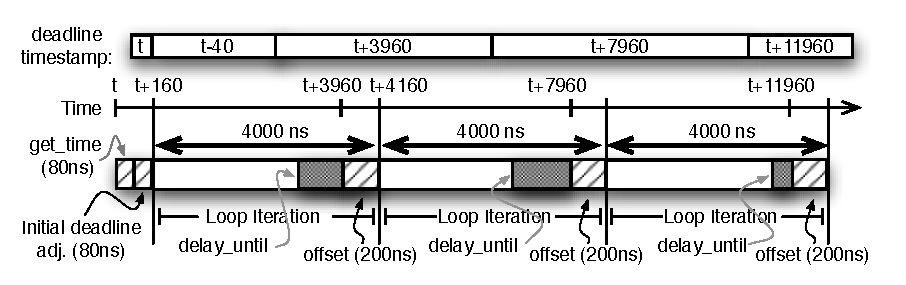
\includegraphics[scale=.9]{figs/setup_loop_timing_adj}
  \end{center}
  \vspace{-3mm}
  \caption{Adjusted timed loop setup}
  \label{fig:setup_look_timing_adj}
\end{figure}

This first iteration jitter can be accounted for by adjusting the initial \deadlinet\ in the loop setup code.
In listing~\ref{lst:timed_loop_compensate_adj} we show an example source code that adjusts for the additional overhead in the loop.
Lines 22 to 25 show the additional loop overhead that conditionally checks whether to branch back to the beginning of the loop.
The offset that we have to adjust for in this example is exactly 200ns, which includes the 4 instructions for the loop overhead and the \delayuntil. 
This offset is reflected on line 9.
Lines 4 to 6 show the loop setup code where we adjust for the execution time of the initial loop iteration, where 40 is subtracted from the initial \deadlinet\ obtained by the \gettime\ on line 4.
This value is obtained by the execution time difference of the overhead, which is $200ns$, and the setup code after \gettime, which is $160 ns$ (4 thread cycles).
We show the resulting timing behavior in figure~\ref{fig:setup_look_timing_adj}, where the first loop iteration is adjusted to 4000ns, the same as subsequent iterations.
By entering the loop with the \deadlinet\ value of $t-40$, we shift the \delayuntil\ deadlines for all loop iterations by 40 ns, allowing us to compensate for the first iteration jitter.   
Intuitively, we adjust the initial \deadlinet\ before entering the loop to create the illusion that the setup code and the loop overhead observed between each \delayuntil\ has the same execution time.
By doing so, the first loop iteration will observe the same loop period as all subsequent iterations. 

\subsection{Exceptions}
In section~\ref{subsec:exception_handling_in_ptarm} we described how exceptions are thrown in PTARM.
When an exception is triggered in one hardware thread, none of the other hardware threads are affected, as the pipeline is not flushed.
For the thread on which the exception occurred, only one thread cycle is lost, and the control flow jumps to the correct exception handler depending on the exception vector table.    
Here, we give a concrete example of the timing properties of exceptions on PTARM by showing how \exceptiononexpire\ and \deactivateexception\ trigger \timerexpired\ exceptions to handle missed deadlines immediately.
The code for the example is shown in listing~\ref{lst:exception-sample}.

\begin{lstlisting}[float=h, label=lst:exception-sample,caption=Sample code that triggers a \timerexpired\ exception ]
  mov  r3, #0x98              ; r3 = address of _timer_handler_loc 
  add  r4, pc, #32            ; r4 = addr of delay_handler
  str  r4, [r3]               ; register delay_handler
  
  cdp  p13, 8, c2, c0, c0, 0  ; get_time
  adds r3, #240
  adc  r2, #0
  cdp  p13, 2, c2, c2, c3, 0  ; exception_on_expire
  
  add  r5, r6, r6             ; arbitrary code block
  add  r7, r5, r6             ;
  
  cdp  p13, 5, c8, c2, c3, 0  ; deactivate_exception
  b end_program                       
  
delay_handler:
  mov pc, lr                  ; simply return
\end{lstlisting}

\newcommand{\delayhandler}{\emph{delay\_handler}}
\newcommand{\Delayhandler}{\emph{Delay\_handler}}
\newcommand{\timerhandlerloc}{\emph{\_timer\_handler\_loc}}

In this example, a \delayhandler\ is setup on lines 16 and 17 that simply returns when called.
\Delayhandler\ is registered as the exception handler for the \timerexpired\ exception, which happens on lines 1 to 3.
This is done by deriving the address of the \delayhandler\ on line 2, and storing it to the \timerhandlerloc.
The \timerhandlerloc\ is a reserved location that points to the address of the handler that is executed when the \timerexpired\ exception is thrown.
When a \timerexpired\ exception is thrown, the current address is saved and control flow jumps to the exception table entry for the \timerexpired\ exception.
This table entry redirects the execution to a \timerexpired\ exception setup code (shown in listing~\ref{lst:timer-expire-handler}) which calls the registered exception handler.
The setup code loads the address of \timerhandlerloc\ into a register, and jumps to the handler on line 7.
If the handler returns, lines 8 to 10 re-enable interrupts, and line 11 returns control to the original PC when the exception occurred.  
\begin{lstlisting}[float=h, label=lst:timer-expire-handler,caption=The \timerexpired\ exception setup code]
.text
.global _tmr_exp_setup;
_tmr_exp_setup:
    push  {r0, lr}                 ; push registers to stack
    ldr   r0, _timer_handler_loc   ; load address of timer expired exception handler
    mov   lr, pc                   ; get return address after calling handler    
    mov   pc, r0                   ; jump to exception handler
    
    mrs   r0, cpsr                 ; get CPSR 
    bic   r0, r0, #0x80            ; enable interrupts
    msr   cpsr, r0                 ; write to CPSR
    pop   {r0, pc}                 ; pop stack and return from exception

_timer_handler_loc: .word  0x00000000;
\end{lstlisting}

The execution trace of this example is shown in table~\ref{table:exception-expire-timing}.
\begin{table}[h]
\begin{center}
\noindent\makebox[\textwidth]{%
\begin{smalltabular}{ | c | c | l | l r | }
  \hline                        
  Time & TC & Address & Inst & Comment\\ \hline
  t ns & n & 0x40000000 & \textit{mov r3, \#0x98} & gets the \timerhandlerloc \\  
  t+40 ns & n+1 & 0x40000004 & \textit{add r4, pc, \#32} & get \delayhandler address \\
  t+80 ns & n+2 & 0x40000008 & \textit{str r4, [r3]} & register \delayhandler as timer expire handler\\
  t+120 ns & n+3 & 0x40000014 & \textit{cdp p13, 8, c2, c0, c0, 0} & get\_time (timestamp: t+120) \\
  t+200 ns & n+5 & 0x400000C & \textit{adds r3, \#240} & timestamp += 240 \\
  t+240 ns & n+6 & 0x40000010 & \textit{adc r2, \#0} & timestamp: t+360 \\
  t+280 ns & n+7 & 0x40000018 & \textit{cdp p13, 2, c2, c2, c3, 0} & exception\_on\_expire, input timestamp: t+360 \\
  t+320 ns & n+8 & 0x4000001C & \textit{add r5, r6, r6} & code block\\
  t+360 ns & n+9 & 0x40000020 & **throw exception** & timer expired, hardware exception thrown\\  
  t+400 ns & n+10 & 0x1C & \textit{b \_tmr\_exp\_setup } & branch to setup code \\  
  t+440 ns & n+11 & 0x78 & \textit{push \{r0, lr\}} & push registers to stack\\
  t+560 ns & n+14 & 0x7C & \textit{ldr   r0, \_timer\_handler\_loc} & load address of timer expired handler \\
  t+600 ns & n+15 & 0x80 & \textit{mov   lr, pc} & store return address after timer handler \\
  t+640 ns & n+16 & 0x84 & \textit{mov   pc, r0} & jump to handler (\delayhandler) \\
  t+680 ns & n+17 & 0x4000002C & \textit{mov   pc, lr} & \delayhandler\ code, return\\  
  t+720 ns & n+18 & 0x88 & \textit{mrs   r0, cpsr} & get CPSR\\
  t+760 ns & n+19 & 0x8C & \textit{bic   r0, r0, \#0x80} &  enable interrupts\\
  t+800 ns & n+20 & 0x90 & \textit{msr   cpsr, r0} &  write to CPSR\\
  t+840 ns & n+21 & 0x94 & \textit{pop   \{r0, pc\}} & pop stack and return from exception\\
  t+960 ns & n+24 & 0x40000020 & \textit{add r7, r5, r6} & re-execute instruction \\
  t+1000 ns & n+25 & 0x40000024 & \textit{cdp p13, 3, c2, c0, c1, 0} & \deactivateexception\ (does nothing) \\
  t+1040 ns & n+26 & 0x40000028 & \textit{b end\_program} & jump to end of program \\
  \hline 
\end{smalltabular}}
\end{center}
\caption{Exception\_on\_expire sample code timing details}
\label{table:exception-expire-timing}
\end{table}
Because execution jumps back and forth between the main code, the \timerexpired\ setup code, and the \delayhandler, so we show the address of the instructions to help follow which code segment is being executed.
The user code is compiled to start at 0x40000000, which is the instruction scratchpad space for hardware thread 0, which we assume this code is running on.
As described in section~\ref{sec:ptarm_memory}, the exception vector table and \timerexpired\ setup code are all compiled to the memory space of the boot ROM.
The \emph{str} instruction is storing to the \timerhandlerloc, which also resides in the boot ROM, so executes in one thread cycle.  
The deadline timestamp is set so the timer expired exception is thrown during the execution of the code block, which occurs at time $t+360$.
Although the address of execution at that time is 0x400000020, the instruction at that address does not complete, because the \timerexpired\ exception is thrown in that thread cycle.
That address is saved to the \emph{link register} (R14) in hardware when the exception is thrown.
The very next thread cycle, the exception vector entry for the \timerexpired\ entry (at address 0x1C) is executed. 
The entry forces a branch to the \timerexpired\ setup code, which executes to call the \delayhandler, the registered the exception handler.       
The \emph{push} and \emph{pop} instructions are load/store multiple instructions that load to the stack, which is located on the data scratchpad. 
These instructions update the base register, and are operating on 2 registers each, so they both take 3 thread cycles to execute.
In section~\ref{subsec:exception_handling_in_ptarm} we discussed the potential execution variability for memory operations if the instruction interrupted by the exception is a long latency memory operation to the DRAM. 
In order to maintain a deterministic execution time for all memory operations, the compiler ensures that the first four thread cycles (the DRAM access latency) after an exception is thrown does not access the DRAM. 
The exposed memory hierarchy with scratchpads allows us to statically compile the exception setup code and data stack, both accessed right after an exception is thrown, onto the scratchpad. 
This ensures that the DRAM is not accessed during the first four thread cycles after the exception is thrown.

The timing analysis of exceptions thus is straightforward in the PTARM architecture.
No flushing of the pipeline occurs, no other hardware threads are affected, and the hardware exception mechanism only has a one thread cycle hardware overhead.
Due to deterministic instruction execution time and exposed memory hierarchy, the \emph{response time} of hardware exceptions, which is the time elapsed between when the exception is thrown and when the user registered exception handler is executes, is deterministic and can be statically obtained. 
For the \timerexpired\ exception in PTARM, the response time is 8 thread cycles ($320ns$), which is reflected in table~\ref{table:exception-expire-timing}.



